%!TEX root = ../main.tex
\chapter{纳米结构表面光阴极发射特性研究}
\label{chap:NPC}

如绪论中所述,光阴极表面的粗糙度可能对热发射度造成影响,降低束流亮度。那么是否可能利用表面粗糙度对阴极上束流的品质进行提高呢?随着纳米加工技术的提高,近年来多个实验室(LBNL,UCLA 的 Pegasus 实验室等)对这种可能性进行了一定探究,即在金属阴极表面加工上纳米纹理,使入射激光激励起表面等离激元\cite{Polyakov:2013aa,Li:2013aa}。表面等离激元可以极大地增强光子吸收效率,也就是加强了金属的量子效率;同时光子被囚禁在阴极表面形成极高的激光功率密度,如果采用单光子光电效应,那么发射电荷量可以成倍数提高;若采用多光子光电效应,那么根据多光子光电发射的特征 $J \propto I^n$,可知发射电荷量可成量级地提高\cite{Li:2013aa}。

针对铜表面纳米阴极的实验研究已经陆续开展了一些\cite{Polyakov:2013aa,Li:2013aa},并已在实验中观察到上百倍的电子产额增益\cite{Li:2013aa}。目前的实验中均采用铜作为纳米表面阴极的基底,这主要考虑到铜的易于获得和加工的特性。本章我们探索了几种新材料:银,镁,镍等作为表面纳米阴极基底的可能性。如前所述,纳米表面阴极相较于传统光滑表面阴极有着电子产额高的优势;然而由于表面上的纳米结构的存在,其发射度必然会受到影响;要衡量纳米表面阴极作为光阴极的潜力必须对其进行综合的测试。本章就通过实验,来探究新材料纳米表面阴极的实际表现。

\section{表面等离激元与纳米表面光阴极}
\subsection{表面等离激元}
纳米表面阴极是利用其表面上产生的表面等离激元 SPPs(也可写成 Surface Plasmons,SPs)进行光电发射的,本节简单介绍 SPs 的性质。
\subsubsection{SPs 的本质}
SPs 是发生在两种材料交界面处的相干电子振荡模式(参见图 \ref{fig:SPs})\cite{Ritchie:1957aa},当这种相干电子振荡模式与入射到两种材料交界面的光子耦合时,便产生表面等离激元,SPs 可沿交界面传输。SPs 是由于电磁波因与材料中的自由电子相互作用,而被束缚在交界面上传播而产生的,它既不是纯粹的电荷振荡模也不是单纯的电磁波,而是由这两者组成。正因为这种混合的机制,称其为 SPPs 更加准确。并不是所有材料交界面处都能产生 SPs,SPs 产生的必要条件是:两种材料的介电常数的实部反号。

满足这个条件的常见的材料组合是金属和电介质。
\begin{figure}[htbp]
\centering
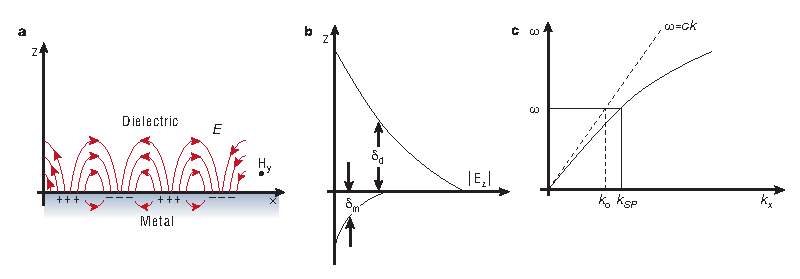
\includegraphics[width=0.9\textwidth]{SPs}
\caption{\label{fig:SPs} SPs 示意\cite{Barnes:2003aa}。a:SPs 的产生与传播;b:SPs 的电磁场场强分布;c:SPs 的色散关系}
\end{figure}

因为在金属中,其中的电子以电子气的形式存在,其内部本质上是等离子体。不考虑损耗时,金属的相对介电常数可以写做:
\begin{equation}
\varepsilon(\omega) = 1-\dfrac{\omega_P^2}{\omega^2}
\label{equ:metal}
\end{equation}
其中 $\omega_P$ 是金属的等离子体频率,即:
\[
	\omega_P = \sqrt{\dfrac{ne^2}{\varepsilon_0m^*}}
\]
因此当金属中电磁波的 $\omega<\omega_P$ 时,金属的介电常数就是负数。而一般电介质(比如空气)的介电常数是正实数,这就满足了 SPs 的产生条件。

考虑了金属的欧姆损耗后,金属的相对介电常数可以写为\cite{wikipedia:aa}:
\begin{equation}
\label{equ:e}
\varepsilon = \varepsilon^{\prime} + i\varepsilon^{\prime\prime}
\end{equation}
其中实部 $\varepsilon^{\prime}$ 就是式 \ref{equ:metal} 中的形式,而虚部 $\varepsilon^{\prime\prime}$ 就造成了 SPs 的传输长度的存在(若无损耗,SPs 可以沿着金属表面传输到无穷远)。

\subsubsection{SPs 的激发}
SPs 可以用电子或者光子激发\cite{Novotny:2012aa}。电子激发即将电子束射入金属,射入金属的电子会发生散射,损失的能量就提供给金属内部的等离子体,散射矢量的平行于金属表面的分量就会形成 SPs。
\begin{figure}[htbp]
\centering
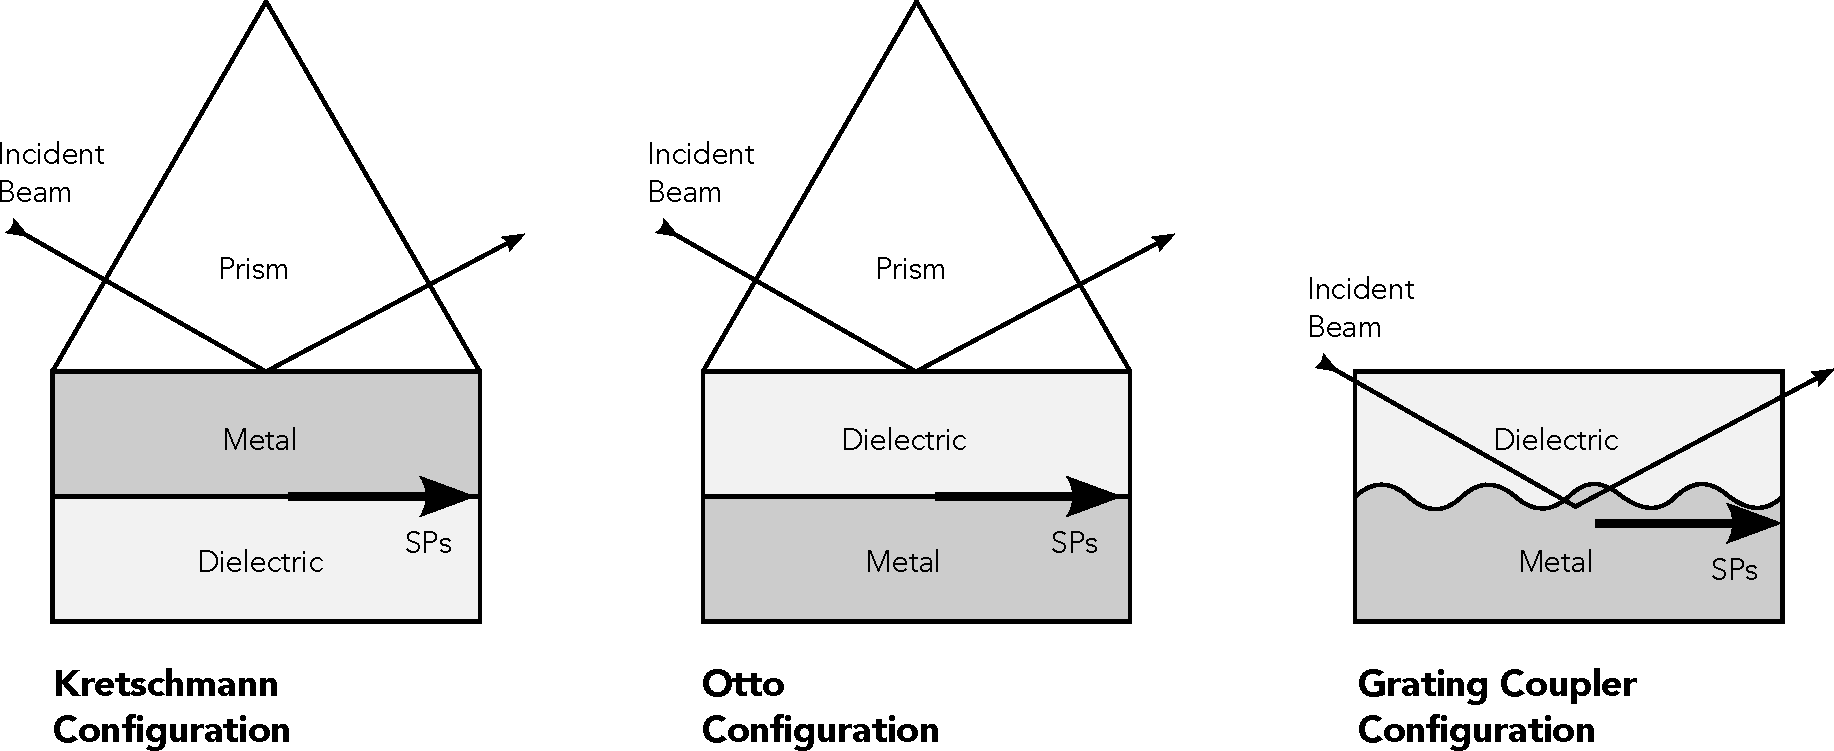
\includegraphics[width=0.9\textwidth]{excitation}
\caption{\label{fig:exc} 光子激发 SPs 的三种方式}
\end{figure}

下面重点讨论光子激发。为了使光子能够激发 SPs,必须将光子与 SPs 模式耦合起来,也就是形成 SPPs。光子激发有三种常用的激发方式:Kretschmann 构型,Otto 构型以及光栅耦合器构型\cite{Novotny:2012aa},参见图 \ref{fig:exc}。

三种激发方式的原理都是通过耦合装置,使入射光子的波矢量的平行(于金属表面的)分量与 SPs 的波矢量的平行分量相等,进而令二者发生持续的能量交换,即发生耦合。表面纳米阴极就是依靠最后一种光栅耦合器的原理进行 SPs 激发的。

\paragraph{以棱镜为耦合器}
后面会说明,SPs 的色散曲线始终在光的色散曲线的右边,因此相同频率的 SPs 和光相比,SPs 的波数一定比光的波数大,无法直接耦合\footnote{典型值是:银和空气的交界面上存在的 SPs 模式的波数 $k_{\text{SP}}\approx 1.03k_0$}。参见图 \ref{fig:exc},光在通过棱镜后,其平行于金属表面的动量会增大(也即波数增大,$p=\hbar k$),这样就可能使光的横向波数与 SPs 模的横向波数匹配。Kretschmann 构型与 Otto 构型就采用这种原理来激发 SPs。需要注意的是,Kretschmann 构型中的金属层是金属薄膜,而 Otto 构型中的介质层一般是一个极小的气隙。

\paragraph{以金属表面光栅为耦合器}
金属表面的周期性波浪结构(表面光栅)存在着空间周期,因此具备波数 $k_{\text{grating}}$,光栅耦合器就是利用金属表面的波数来增加光的横向波数,使 SPs 模式与光耦合起来形成 SPPs。假设光栅的空间周期为 $a$,那么\cite{Novotny:2012aa}:
\[
	k_{\text{SP}} = k_{\text{x, photon}} \pm nk_{\text{grating}} = k_0\sin\theta_0 \pm n\dfrac{2\pi}{a}
\]
其中 $k_0$ 为真空中光的波数,$\theta_0$ 是光的入射角,$n$ 是谐波数。可见,金属的表面光栅如果取适当的空间周期,就可以将以某些角度入射的光子与 SPs 耦合起来。

\paragraph{以粗糙金属表面为耦合器}
前面说明了使用金属表面光栅为耦合器的原理,那么不难理解一般的粗糙金属表面也可以做为耦合器:粗糙的金属表面可以看成由许多空间周期不同的光栅叠加而成。入射角不同的入射光,会选择相应的光栅分量来增加自己的横向波数,进而与 SPs 耦合。

对于随机的粗糙金属表面,由于其各个空间周期的光栅分量都存在,因此理论上可以与以任意入射角入射的光子耦合成 SPP。但是每一个 SPP 模式强度都不大。可以操控金属表面形态,使其耦合出特定的 SPP 模式,这也是等离激元电路(Plasmonic Circuit)的基础。

\subsubsection{SPs 的主要性质}
SPs 有一些非常直观的重要性质。它沿交界面的法向是渐消的,而在平行交界面的方向是传播的,这就是 SPs 最重要的性质:只沿交界面传输,因此 SPs 的能量不会因辐射而损失。但是其能量仍然会在金属表面因欧姆损耗而耗散,所以这就决定了 SPs 不可能沿交界面无限地传输下去,就有传输长度的概念。

在我们最关心的粗糙金属表面情况下,发现纳米级的周期性表面缺陷(周期性凸点,条带等)结构会使 SPs 的色散曲线断裂形成禁带,可以利用这一点来限制 SPs 的传播范围,进而形成真正的电路。

\paragraph{色散关系}
SPs 的色散曲线请参见图 \ref{fig:SPs}c,其色散关系为:
\begin{equation}
\label{equ:disp}
k_x = \dfrac{\omega}{c}\sqrt{\dfrac{\phantom{|}\varepsilon_1\varepsilon_2\phantom{|}}{\varepsilon_1+\varepsilon_2}}
\end{equation}
若介质 1 是金属,介质 2 是空气或真空,那么:
\[
	k_x = \dfrac{\omega}{c}\sqrt{\dfrac{\omega^2-\omega_P^2}{2\omega^2-\omega_P^2}}
\]
由上式可见,SPs 的色散曲线存在一条平行于 $k$ 轴的渐近线,SPs 模式的频率上限为:
\[
	\omega_{\text{SP}}=\dfrac{\omega_P}{\sqrt{2}}
\]
SPs 色散关系的推导如下。假定介质 1 和介质 2 的相对介电常数分别是 $\varepsilon_1$ 和
 $\varepsilon_2$,那么设两介质交界面处传输的电磁波的电场表达式为:
\[
	E = E_0\exp\big[i(k_xx+k_zz-\omega t)\big]
\]
根据连续性条件,有:
\begin{equation}
\label{equ:c1}
\dfrac{k_{z1}}{\varepsilon_1} + \dfrac{k_{z2}}{\varepsilon_2} = 0
\end{equation}
和介质中的色散关系:
\begin{equation}
\label{equ:d2}
k_x^2 + k_{zi}^2 = \varepsilon_i\left(\dfrac{\omega}{c}\right)^2,\quad i=1,2
\end{equation}
由上面两式便可得到式 \ref{equ:disp}。为了使波只沿表面($x$ 方向)传播,必须使 $k_{z1},k_{z2}$ 为纯虚数,结合式 \ref{equ:disp} 和式 \ref{equ:d2},便可以得到:
\[
	\dfrac{\varepsilon_1\varepsilon_2}{\varepsilon_1+\varepsilon_2} > \max\{\varepsilon_1, \varepsilon_2\}
\]
若认为 $\varepsilon_2$ 是正实数,那么便得出 $\varepsilon_1$ 必须为负,这就得到了前面提到的 SPs 的存在条件:两种材料的介电常数必须反号。

\paragraph{传输长度和趋肤深度}
利用式 \ref{equ:e},考虑了损耗后可以得到 SPs 的复色散关系:
\begin{equation}
\label{equ:cdisp}
k_x = k_x^{\prime}+ik_x^{\prime\prime}= \left[\dfrac{\omega}{c}\left(\dfrac{\varepsilon_1^{\prime}\varepsilon_2}{\varepsilon_1^{\prime}+\varepsilon_2}\right)^{1/2}\right]+\left[\dfrac{\omega}{c}\left(\dfrac{\varepsilon_1^{\prime}\varepsilon_2}{\varepsilon_1^{\prime}+\varepsilon_2}\right)^{3/2}\zskip\dfrac{\varepsilon_1^{\prime\prime}}{2\big(\varepsilon_1^{\prime}\big)^2}\right]
\end{equation}
所以 SPs 的电场为:
\[
	E = E_0\exp\big[i(k_x^{\prime}x+k_zz-\omega t)-k_x^{\prime\prime}x\big]
\]
可见 SPs 的电场沿横向传输的衰减因子为 $\exp(-k_x^{\prime\prime}x)$,而能量与电场的平方成正比,因此 SPs 沿横向传输的能量衰减因子为 $\exp(-2k_x^{\prime\prime}x)$,于是 SPs 模式的传输长度为:
\begin{equation}
\label{equ:l}
\delta_{\text{SP}} = \dfrac{1}{2k_x^{\prime\prime}}
\end{equation}
SPs 的趋肤深度在两种介质中不同,在电介质中的趋肤深度要远大于金属中的趋肤深度。将式 \ref{equ:disp} 代入式 \ref{equ:d2} 中,解出 $k_{zi}$ 便有:
\begin{equation}
\label{equ:z}
\delta_{zi} = \dfrac{\lambda}{2\pi}\left(\dfrac{|\varepsilon_1^{\prime}|-\varepsilon_2}{\varepsilon_i^2}\right)^{1/2}
\end{equation}
通过更仔细的研究可知,SPs 对在趋肤深度内的表面微小扰动非常敏感,因此可以用 SPs 来做金属表面状况的探针。

\paragraph{禁带的产生}
研究发现,当金属表面纳米结构的空间周期 $a$ 满足下式:
\[
	a = \dfrac{\lambda_{\text{SP}}}{2}
\]
其中 $\lambda_{\text{SP}}$ 是 SPs 的有效波长,则散射会导致 SPs 驻波的形成\cite{Barnes:2003aa},这时 SPs 的色散曲线断裂出现禁带,如图 \ref{fig:bg}a 所示。

\begin{figure}[htbp]
\centering
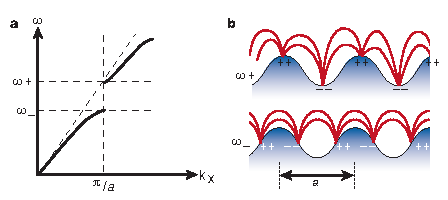
\includegraphics[width=0.65\textwidth]{bandgap}
\caption{\label{fig:bg}禁带形成示意\cite{Barnes:2003aa}}
\end{figure}

禁带形成的原因是,在特定条件下,SPs 会有两个独立的驻波解,这两个驻波解具有相同的波长但频率不同,这两个驻波的频率分别是 $\omega_+$ 和 $\omega_-$,如图 \ref{fig:bg}b 所示,$\omega_+$ 对应的 SPs 波具有更高的能量,因为电荷振荡的幅度更大,且场的扭曲更严重;相反 $\omega_-$ 对应的 SPs 波的能量更低。而频率在两者之间 SPs 波不能传播(衰减模),于是形成了禁带。

由于一维的纳米周期结构会束缚住单一方向传播的 SPs 波,如果采用二维的纳米周期结构,就可能在金属表面全方向上束缚住特定频率范围的 SPs 波,注意到即使是衰减模,其传输长度也足够覆盖数十个表面结构周期,因此这一点可被用来制作等离激元电路。

\subsection{表面等离激元光阴极}
由于 SPPs 有提高入射光吸收率/增强阴极表面光场的性质,可以利用 SPPs 来加强光电发射,提高阴极的量子效率。在金属阴极表面激发起 SPPs,一般采用下面两种方式:
\begin{itemize}
	\item 利用金属表面的光栅结构来提高入射光的横向波数,这种方式对应 NPC(Nano-Patterned Cathode)阴极
	\item 通过将光射入电介质以提高入射光的横向波数,这种方式对应 ATR(Attenuated Total Reflectance)阴极
\end{itemize}

\subsubsection{ATR 光阴极}
在透明电介质上镀一层几十纳米(nm)厚的金属薄膜,就构成了 ATR 光阴极。激光从透明电介质端射入,其横向动量增加,因而能在金属与真空的交界面激发起 SPPs,达到强化光电发射的目的\cite{Sipe:1981aa}。与一般光阴极不同,激光并非是正入射到金属表面,打出反射电子形成光电流,而是背入射到金属表面,其激发的光电子需穿过几十纳米厚的金属薄膜出射而形成光电流。目前 ATR 阴极的实验已经开展了一些,其原理获得了初步验证\cite{Chen:2011aa,Watanabe:2011aa,Neo:2012aa}。
\begin{figure}[htbp]
\centering
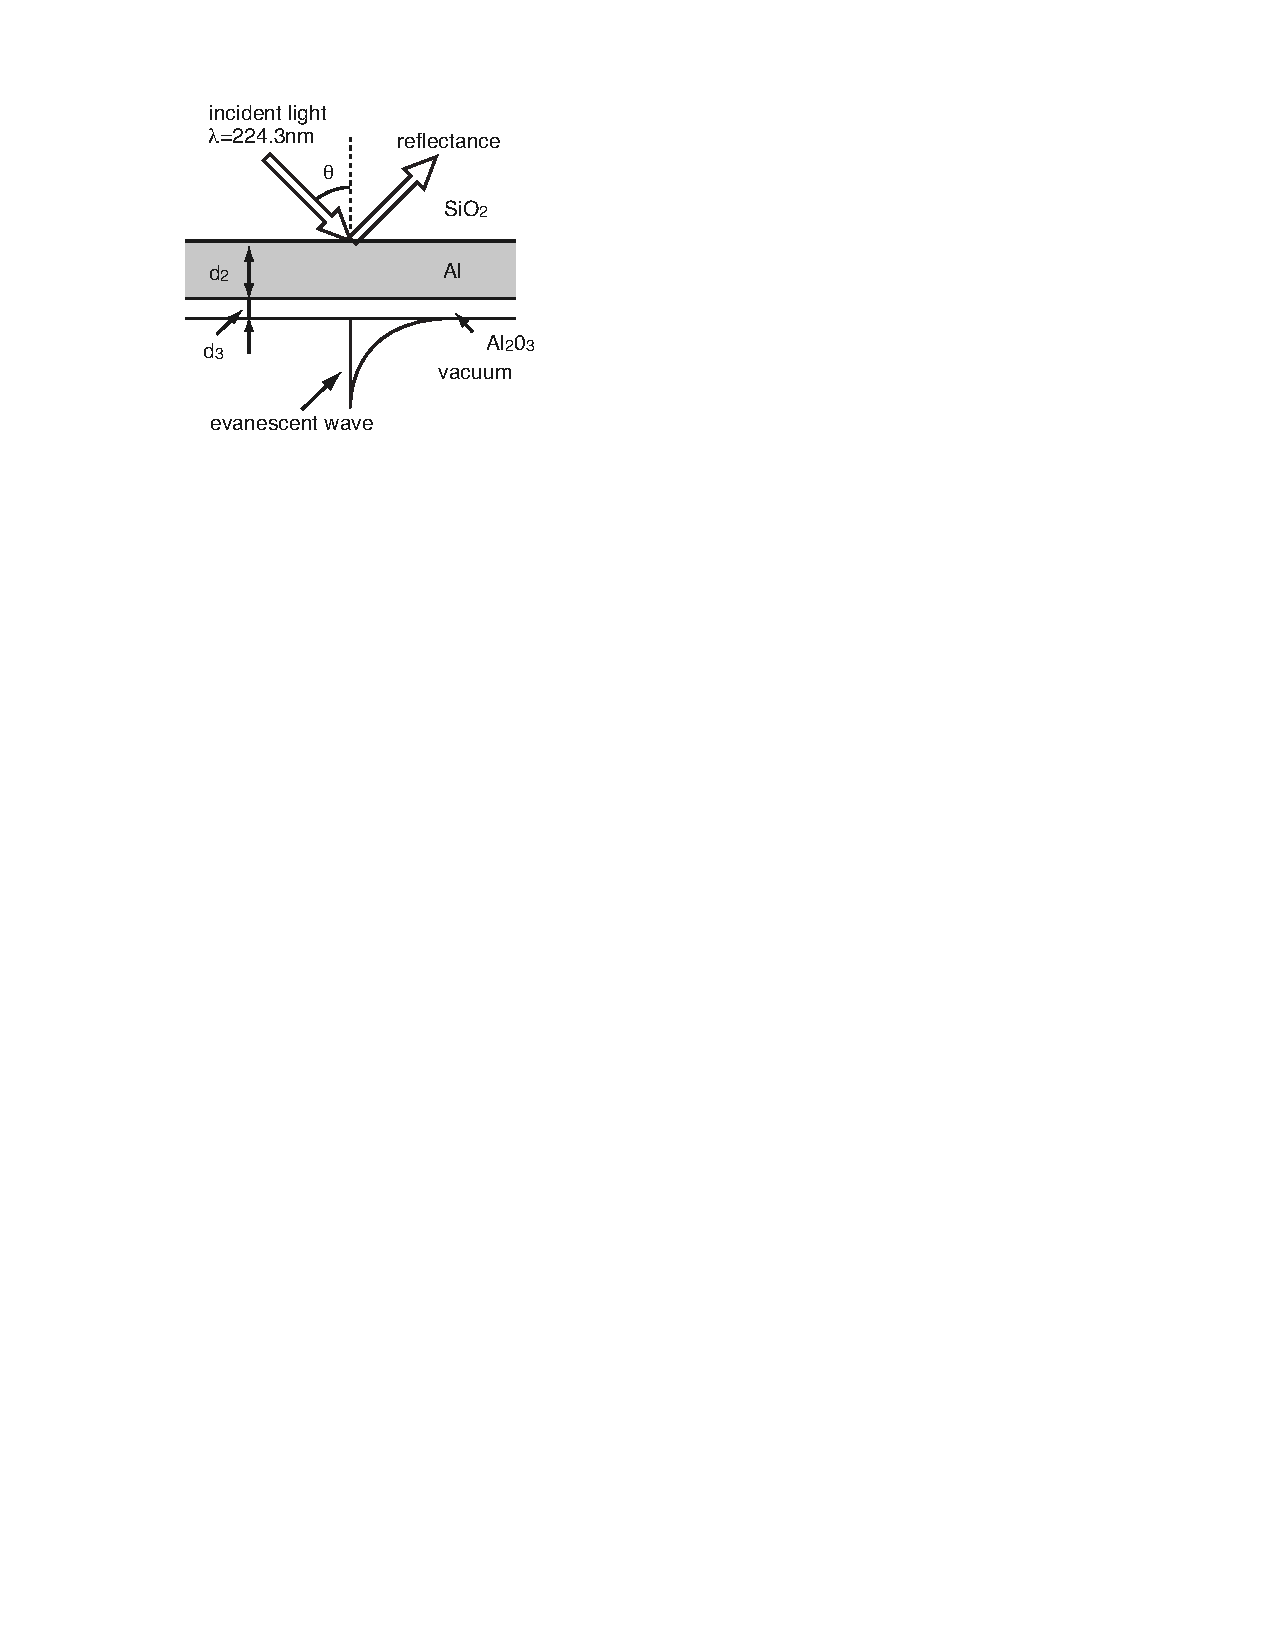
\includegraphics[width=0.6\textwidth]{ATR}
\caption{\label{fig:NPC} ATR 光阴极示意图\cite{Watanabe:2011aa}}
\end{figure}
	
ATR 光阴极具有下面特点:
\begin{itemize}
	\item 量子效率可以比同材料光滑阴极高 1 $\sim$ 2 个量级
	\item 由于电子出射面光滑,发射度与同材料光滑阴极相当
	\item 激光采用背入射方式激发光电子
	\item 应用于微波电子枪时的微波泄漏的问题还需解决
\end{itemize}

\subsubsection{NPC 光阴极}
在金属表面刻上百纳米(nm)级的周期性结构,就构成了 NPC 光阴极。激光入射到该纳米结构(对于激光的作用是反射光栅)时,其横向动量增加,能在表面激发起 SPPs,达到强化光电发射的目的。关于铜纳米表面阴极的实验测量已陆续开展,实验中已观测到上千倍的电子产额增益\cite{Polyakov:2013aa,Li:2013aa}。
\begin{figure}[htbp]
\centering
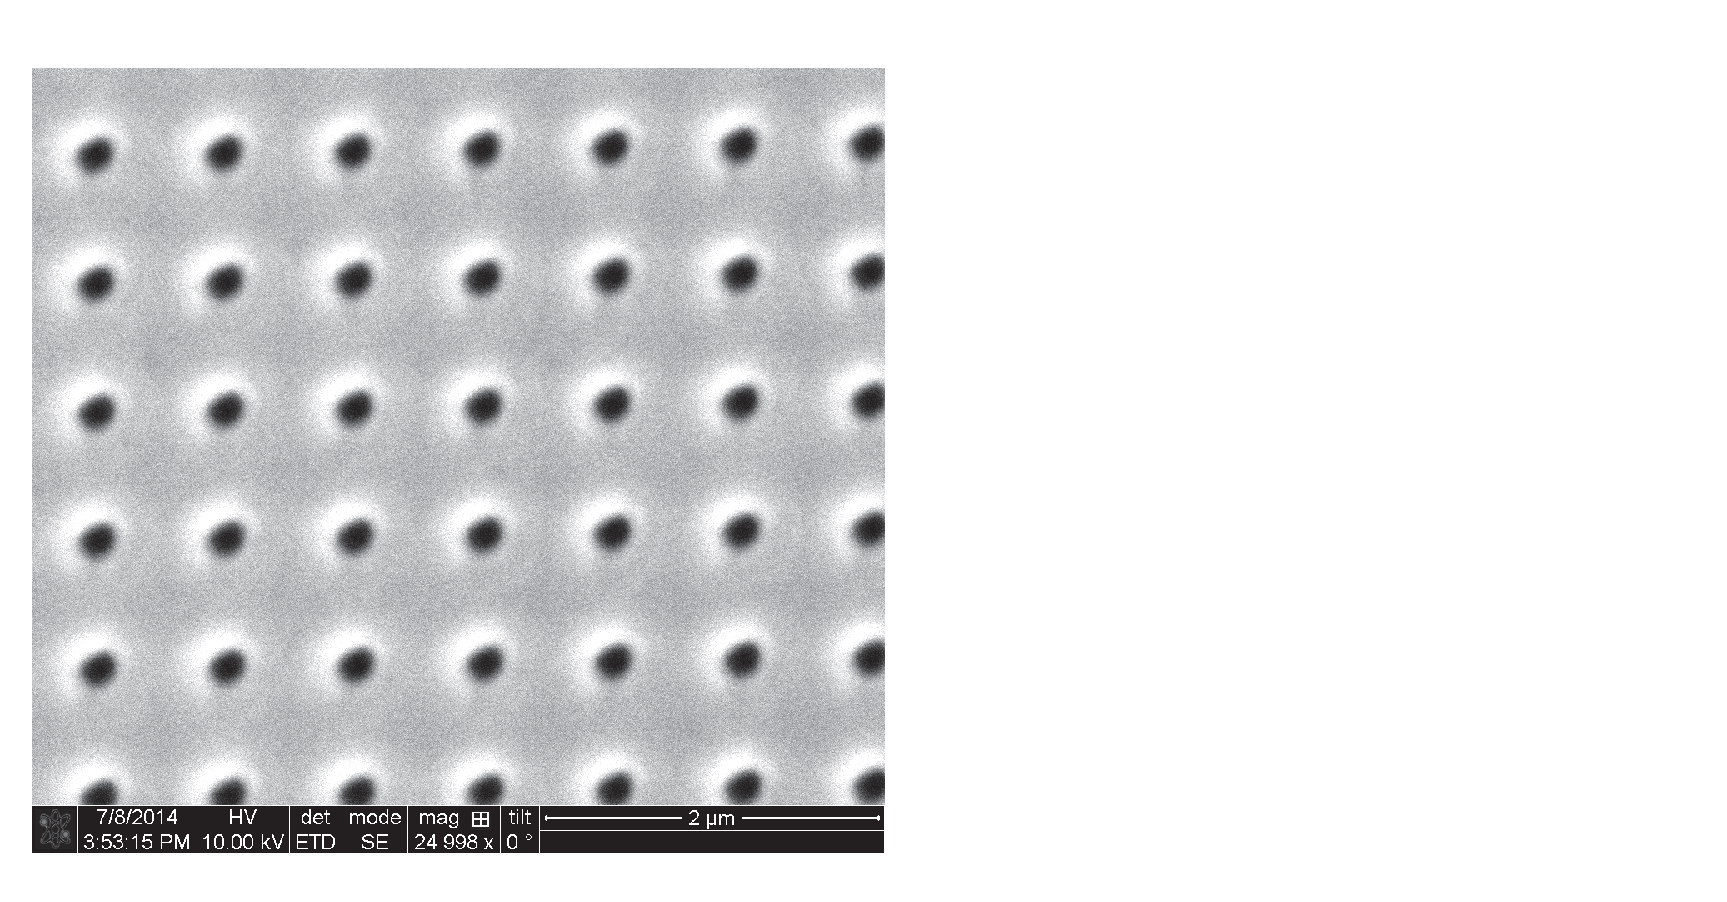
\includegraphics[width=0.5\textwidth]{NPC}
\caption{\label{fig:NPC} NPC 光阴极表面形态}
\end{figure}

NPC 光阴极具有下面特点:
\begin{itemize}
	\item 量子效率可以比同材料光滑阴极高 2 $\sim$ 3 个量级
	\item 由于表面有周期性纳米结构,发射度一般比同材料光滑阴极更大
	\item 多采用多光子光电发射,尽可能利用 SPPs 对表面上激光功率密度的增强
	\item 可直接应用于微波电子枪中
\end{itemize}
本章我们要研究的就是 NPC 光阴极。

\section{纳米表面光阴极的模拟优化\label{sec:sim}}
纳米表面光阴极的独特优势是对入射激光的加强吸收和表面场增强,然而要达到对某波长的激光近乎 100\% 的吸收率,其表面的周期性结构必须经过优化。因此在加工纳米结构之前,首先需要通过数值模拟确定纳米周期阵列的最优尺寸。我们采用了 Lumerical FDTD 程序包\cite{Lumerical:aa}进行表面纳米结构的优化。

\begin{figure}[htbp]
\centering
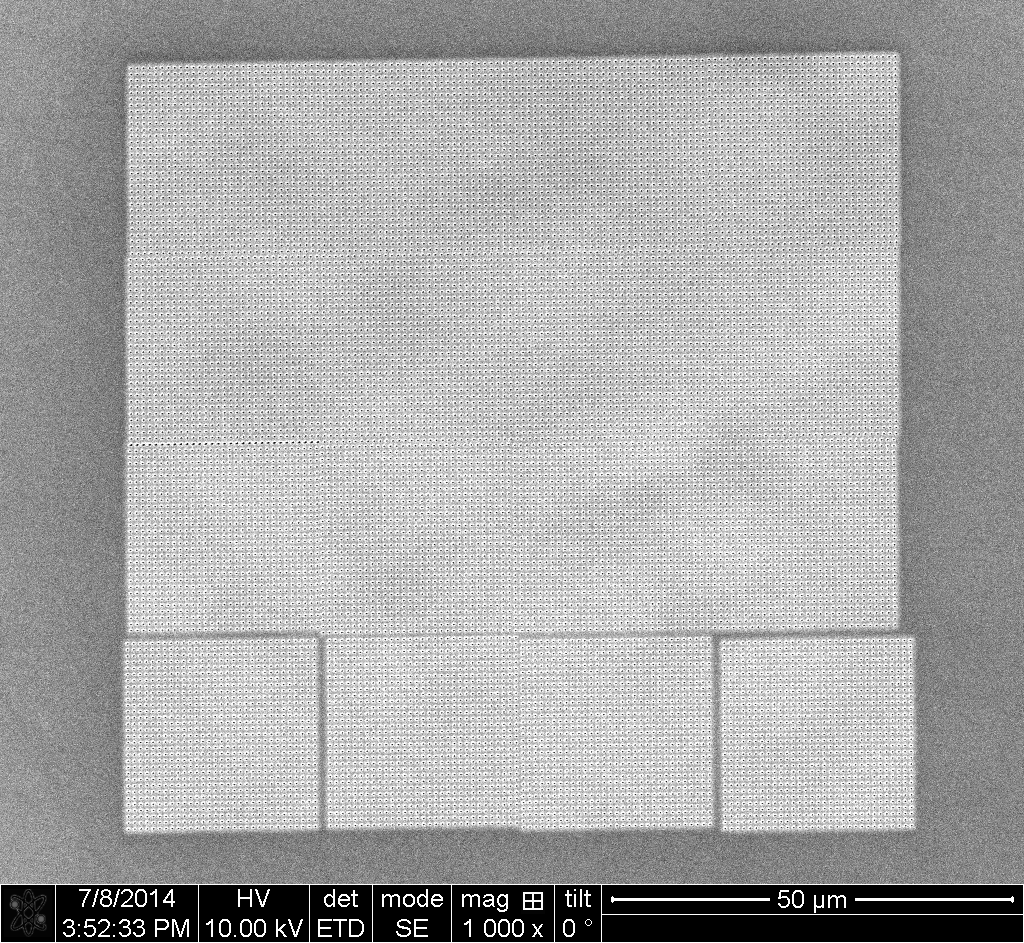
\includegraphics[width=0.45\textwidth]{Cu_ns1}
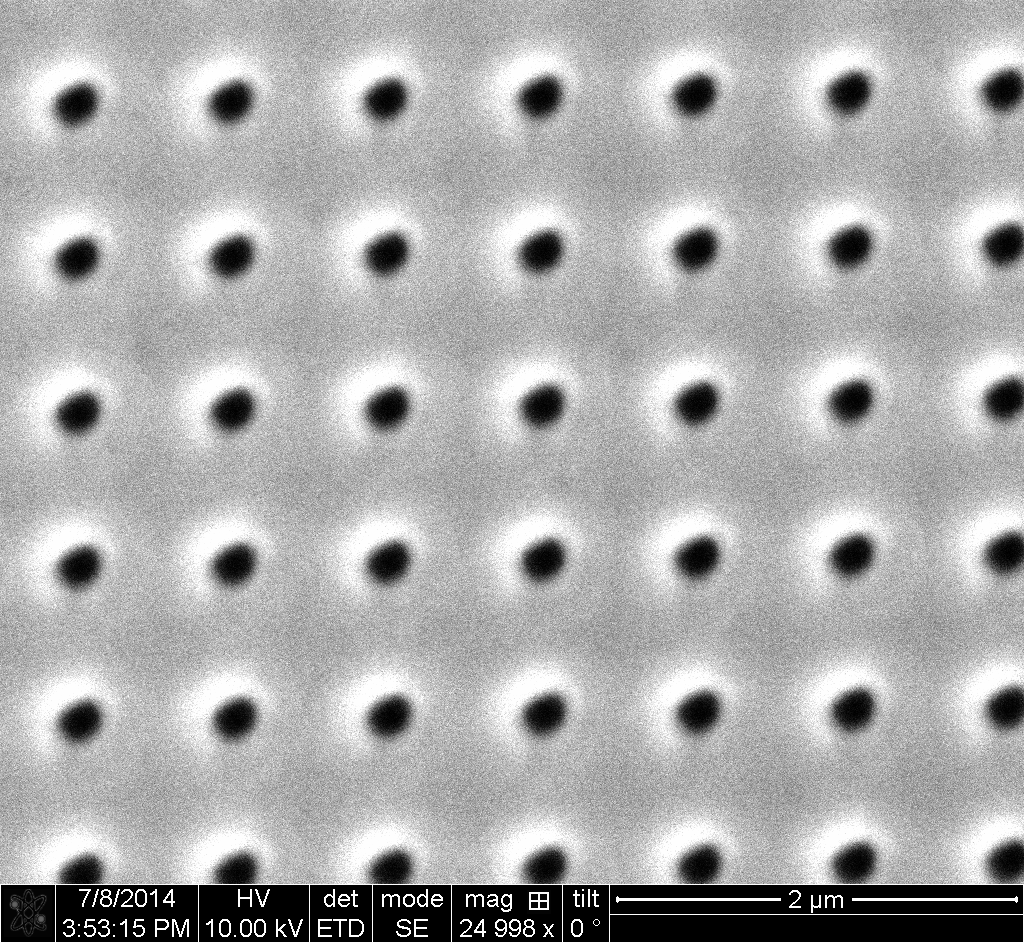
\includegraphics[width=0.45\textwidth]{Cu_ns2}
\caption{\label{fig:Cu_ns_sem} 
铜基底上纳米小孔阵列的原子力显微镜图像。左图:整个纳米阵列形状;右图:单个小孔形状。}
\end{figure}
图 \ref{fig:Cu_ns_sem} 是一张典型的蚀刻了纳米阵列图样的单晶铜晶片。蚀刻的图样是一个二维小孔阵列,其几何属性由四个因素决定:小孔形状,小孔深度,小孔尺寸以及阵列的周期。由于采用了聚焦离子蚀刻法(Focused Ion Beam,FIB)加工小孔阵列,小孔的形状分布接近高斯分布而不能随意变化,且其纵向/横向尺寸比也基本是一个常数($\sim$ 1.2),因此优化的变量就剩下小孔的 rms 宽度 $\sigma$ 及阵列周期。小孔阵列的单个周期轮廓如图 \ref{fig:profile} 中所示。

\begin{figure}[htbp]
\begin{center}
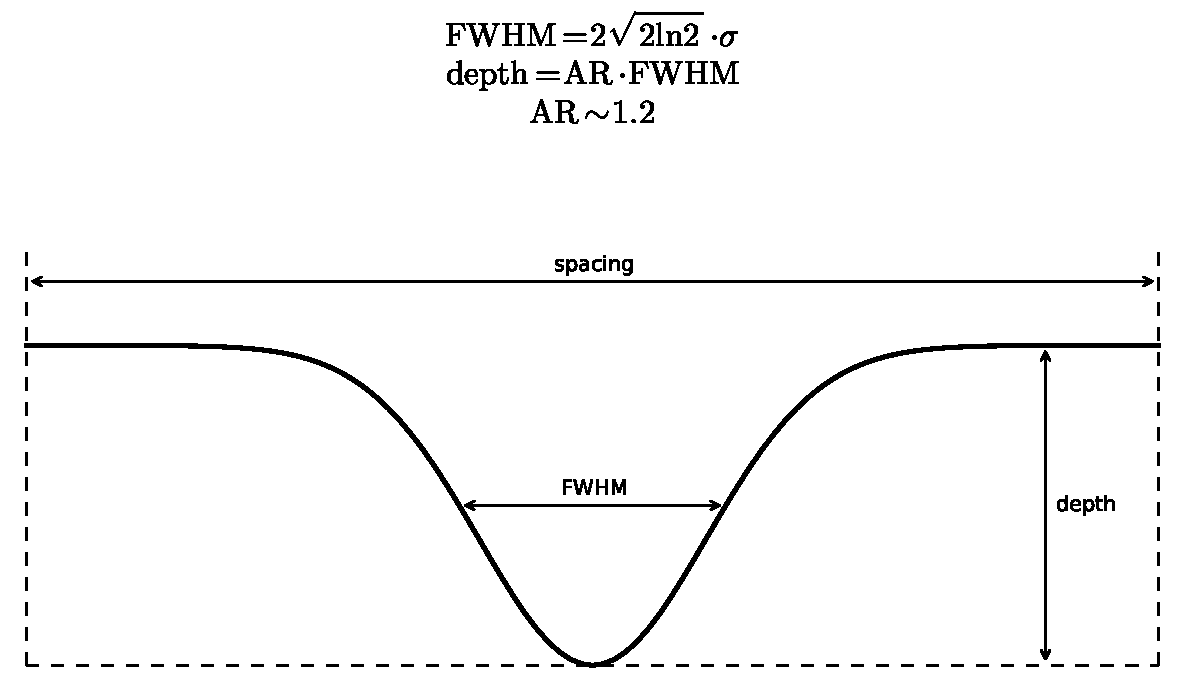
\includegraphics[width=0.47\textwidth]{nanohole}
\caption{\label{fig:profile} NPC 小孔阵列的单周期轮廓}
\end{center}
\end{figure}

在模拟中我们观察到,谐振波长(即使入射激光反射率最小的激光波长)几乎完全由阵列的周期决定。由于实验中我们采用了 掺钛蓝宝石激光器产生的波长 800\,nm 红外激光,在模拟中我们调整阵列的周期,使谐振波长为 800\,nm。小孔的尺寸决定了反射率谱上反射率峰的深度,因此为达到尽可能接近 0 的反射率,该参数也经过了细致扫描。在实验前共准备了四种 NPC 晶片材料,分别是铜,镍,镁和银,对以上四种材料的数值模拟优化结果见表 \ref{tab:opt}。

\begin{table}[htbp]
\caption{\label{tab:opt}几种 NPC 晶片候选材料的阵列几何参数优化结果。模拟中的激光波长为 800\,nm。}
\begin{center}
\begin{tabular}{lllll}
\toprule
材料 & 阵列周期(nm)& 小孔 FWHM(nm)& 小孔深度(nm)& 反射率 \\
\midrule
Cu & 767 & 200 & 240 & 0.40\% \\
Nb & 750 & 280 & 364 & 8\% \\
Mg & 780 & 217 & 261 & 0.81\% \\
Ag & 770 & 174 & 209 & 0.63\% \\
\bottomrule
\end{tabular}
\end{center}
\end{table}
由于铜晶片的 NPC 已经有研究组做过详细实验研究,我们最后选择了反射率次低的银晶片进行进一步加工。选择银也同时考虑到银的逸出功比铜的逸出功低,因此对于相同的激光参数,银阴极有可能产生亮度更高的电子束。

NPC 银晶片加工好后,为评估该银 NPC 的可能表现,首先进行了离线反射率谱测量,之后才可将其集成到电子枪中进行高功率测试。

\section{NPC 离线反射率谱测量}
\subsection{宽谱反射率谱仪}
为实现 NPC 的离线反射率测量,我们设计并搭建了一台宽谱反射率谱仪,该谱仪可以工作在普通实验环境(空气环境)中。反射率谱仪的结构如图 \ref{fig:bbrs} 所示。
\begin{figure}[htbp]
\centering
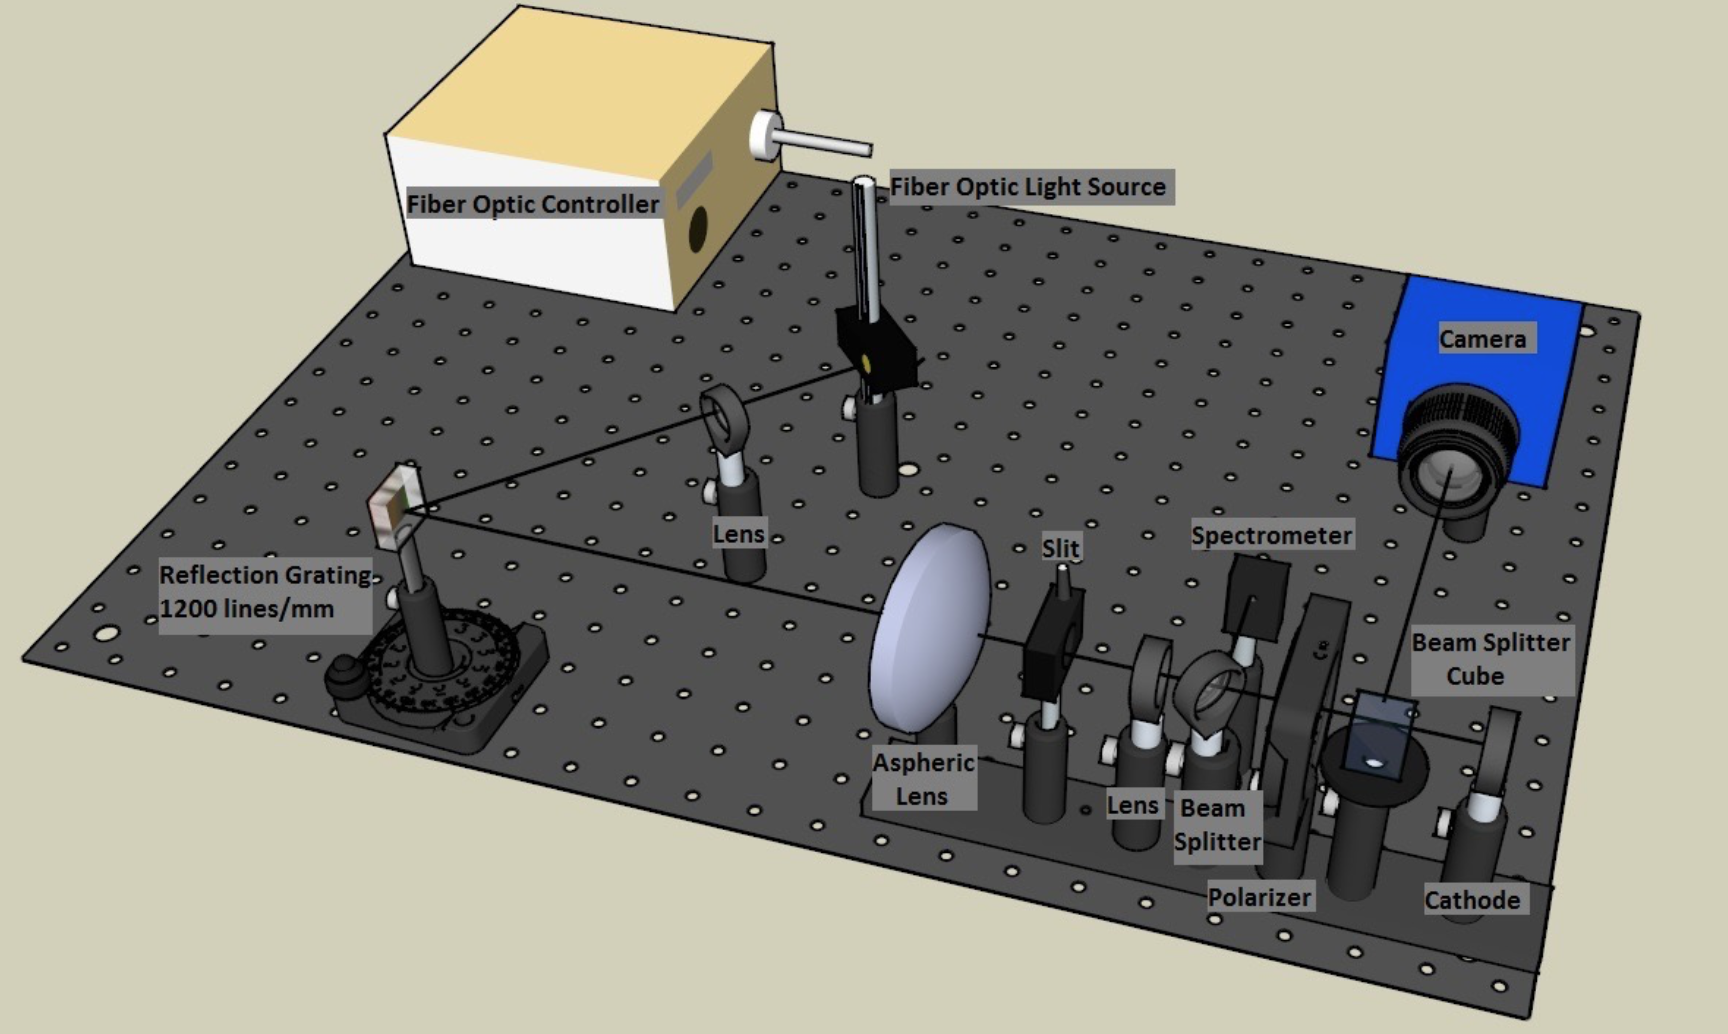
\includegraphics[width=0.6\textwidth]{bbrs.png}
\caption{\label{fig:bbrs} 宽谱反射率谱仪结构图}
\end{figure}

反射率谱仪的原理如下:采用白光高亮度光源产生一束横向尺寸较小的白光,随后该白光入射到一个可转动的反射光栅表面并分光,不同波长的成分其传播方向会不同。分光后较宽的彩色光带会通过一个非球面透镜进行聚焦并使光带传播到一个可调狭缝上,通过调节狭缝的大小可以控制通过狭缝的光的频谱宽度,狭缝越窄,频谱也越窄。被狭缝滤波后的光继续传输,并通过一个分光镜分成等强的两束,其中一束入射到能谱仪上,以测量入射光的带宽;另外一束通过一个可选的偏振片起偏,并通过一个分光块后,最终打在样品上。打在样品上光会被样品反射,进而进入分光块并反射到相机中,相机就可以观察到光打到样品上的反射图像了。由于最初的白光会经过一次狭缝和三次分光,其最后进入相机的强度会显著衰减,为了保证相机图像的信噪比,狭缝不能太小,因此打到样品上的光的带宽也不能太小,经过调整,入射光的 FWHM 带宽可达到 5\,nm 左右,这就是其被称为宽谱反射率谱仪的原因。

\begin{figure}[htbp]
\centering
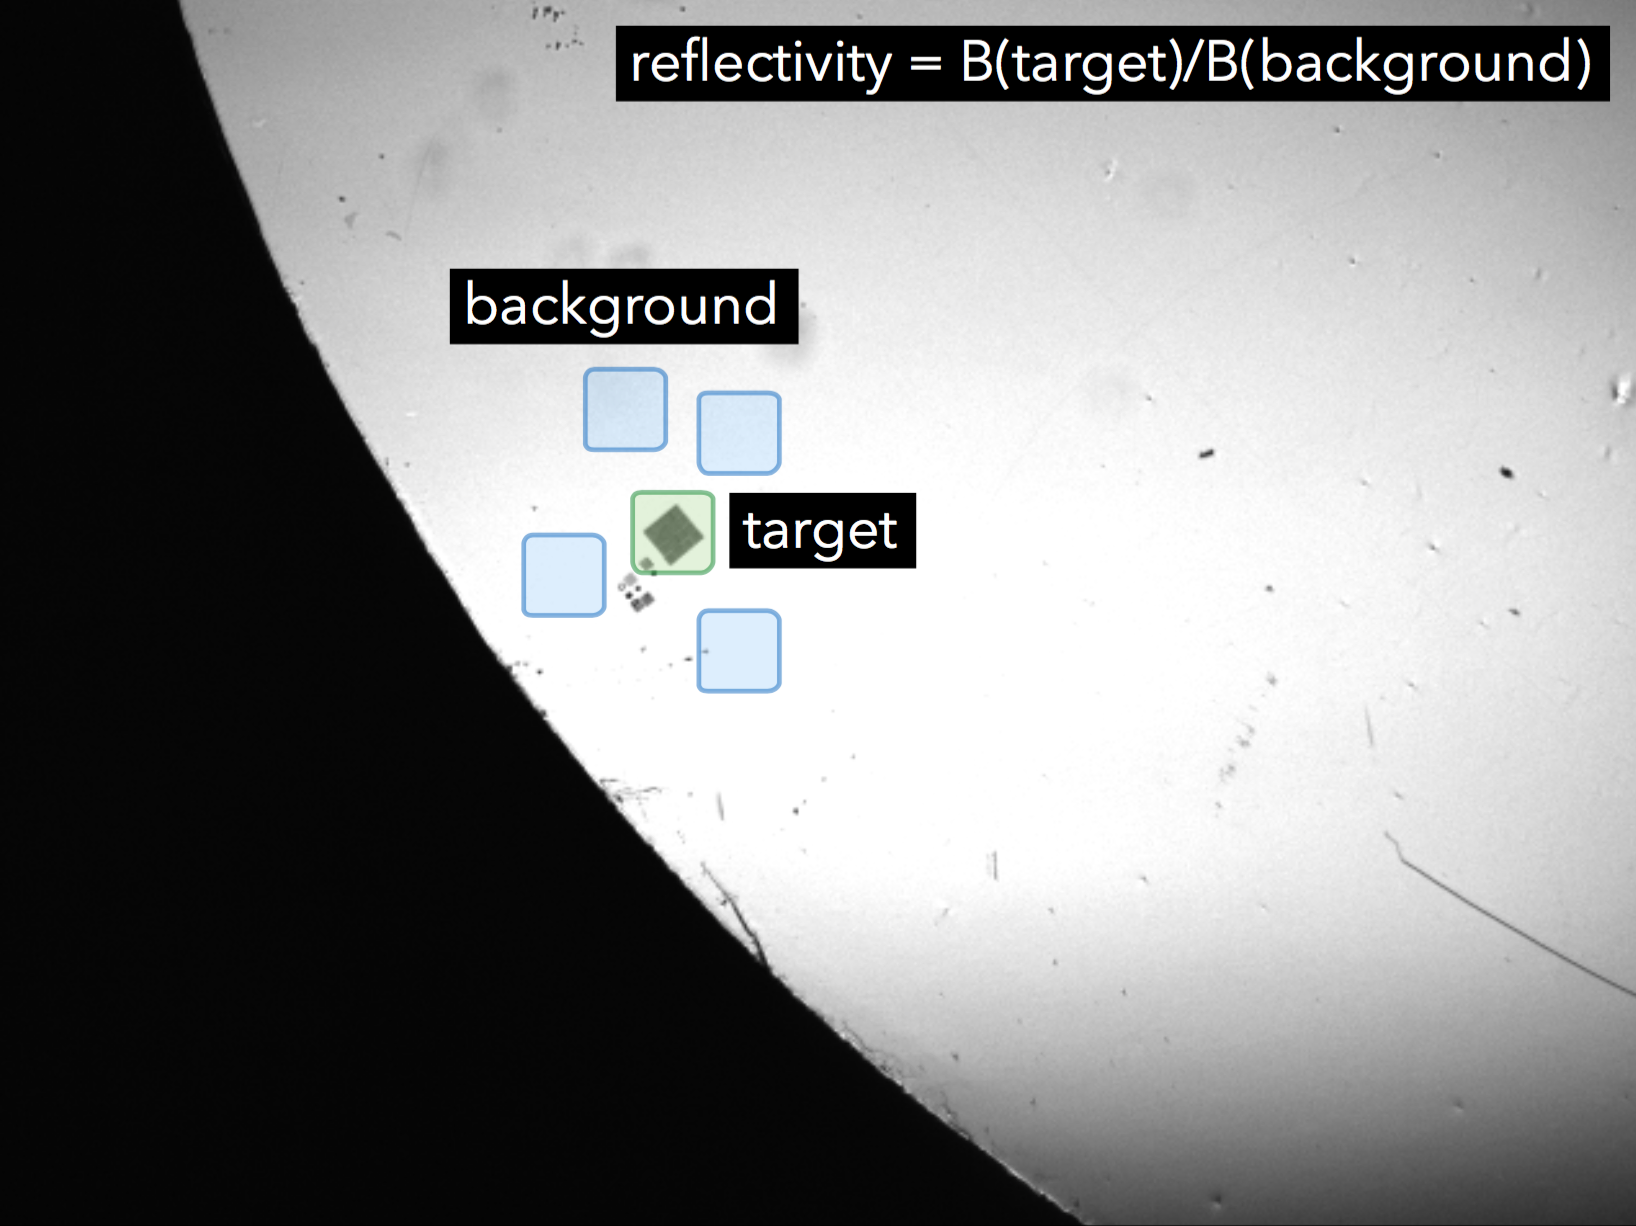
\includegraphics[width=0.45\textwidth]{sample.png}
\caption{\label{fig:sample} 宽谱反射率谱仪测量到的一幅典型 NPC 样品图像}
\end{figure}

图 \ref{fig:sample} 中展示了一张典型的 NPC 样品离线反射率测量图像。在特定中心波长下的纳米结构反射率可通过对图像的分析获得:对图 \ref{fig:sample} 中的蓝色方块中的像素值进行平均,就可获得背景亮度 $B_{\text{bg}}$,对绿色方块中的纳米结构的像素值进行平均,就得到纳米结构的亮度 $B_{\text{pattern}}$,从而在该中心波长下的 NPC 反射率 $R$ 就由式 \ref{eq:ref} 给出:
\begin{equation}
\label{eq:ref}
R = \frac{B_{\text{pattern}}}{B_{\text{bg}}}
\end{equation}

为了获得 NPC 样品较完整的反射率谱,我们可以旋转反射光栅来改变通过窄缝的光束的中心波长。遍历全部感兴趣的光谱区域并记录对应的 NPC 图像,就可以获得该纳米结构晶片的反射率谱。

\subsection{银晶片的反射率谱}
根据 Lumerical FDTD 模拟给出的优化结构参数,我们在单晶银晶片上加工了纳米阵列结构。加工好的阵列形态的 SEM 图像如图 \ref{fig:Ag_b_sem} 所示。
\begin{figure}[htbp]
\begin{center}
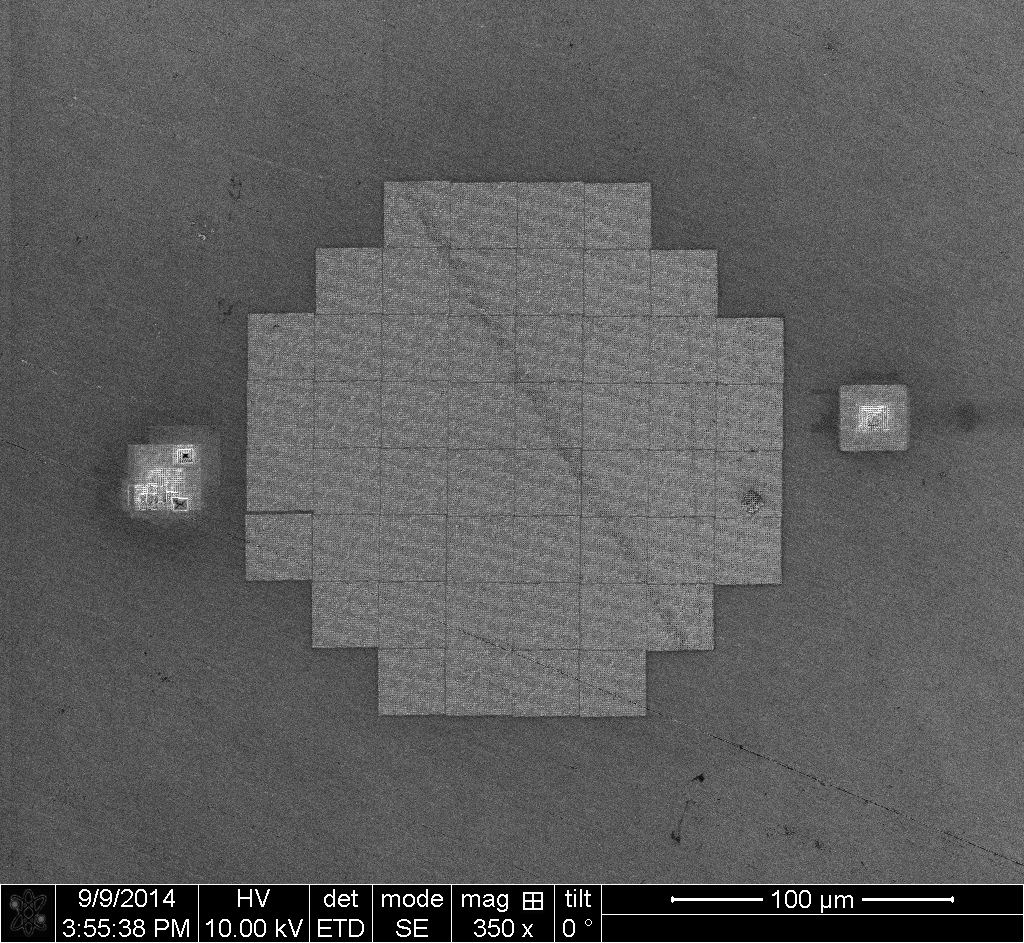
\includegraphics[width=0.45\textwidth]{Ag-b1}
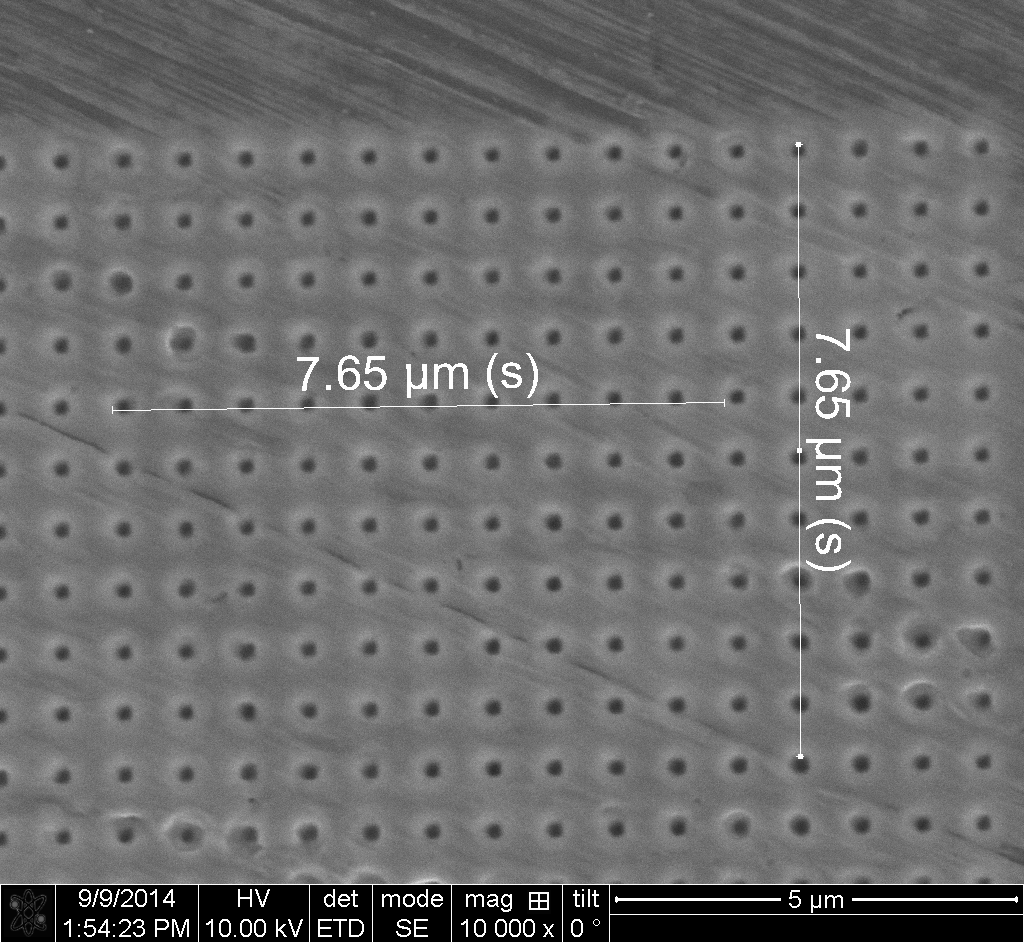
\includegraphics[width=0.45\textwidth]{Ag-b2}
\\[2pt]
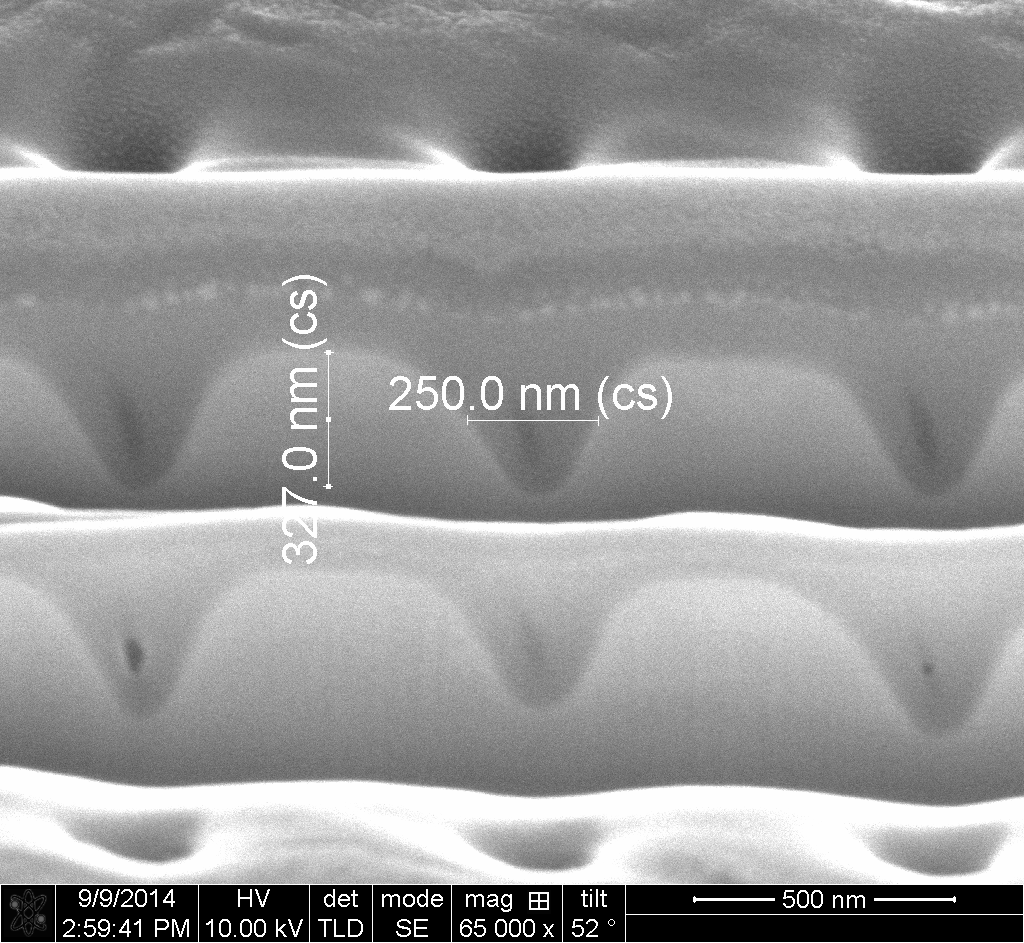
\includegraphics[width=0.45\textwidth]{Ag-0}
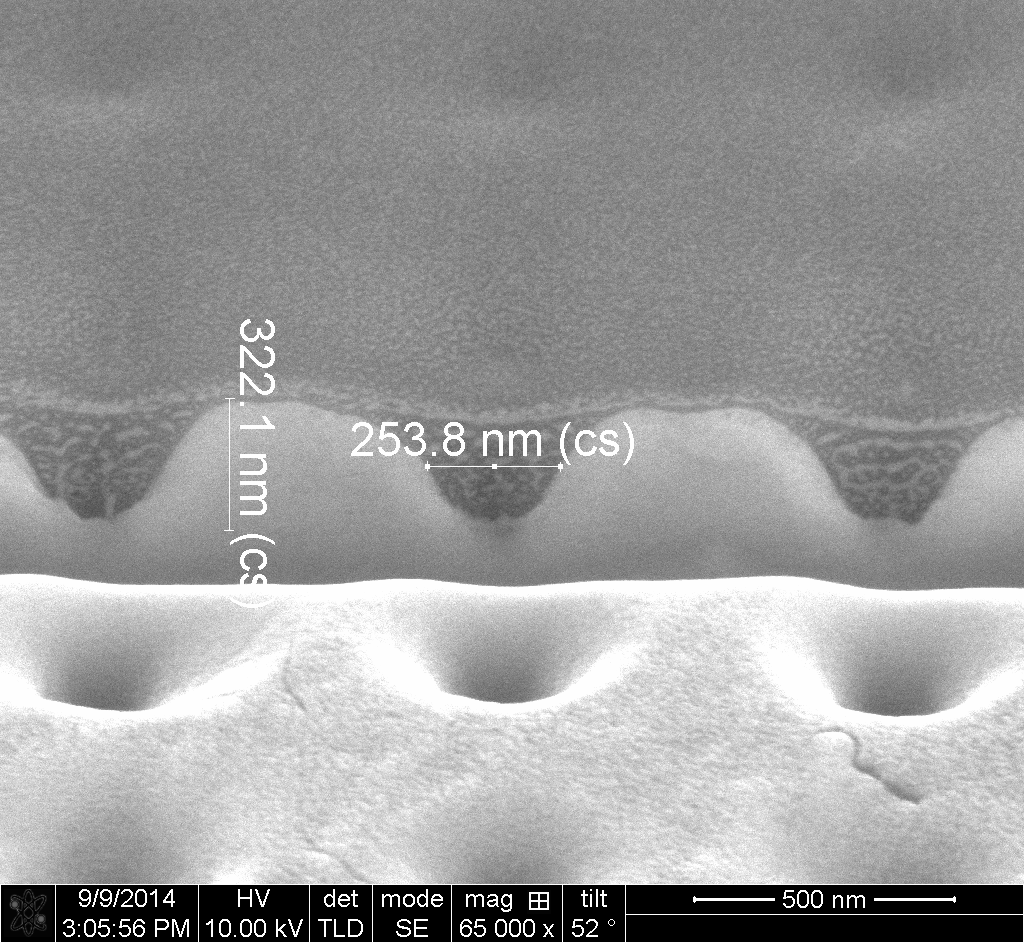
\includegraphics[width=0.45\textwidth]{Ag-90}
\caption{\label{fig:Ag_b_sem} 
纳米结构银晶片表面形态的 SEM 测量结果。左上:阵列的整体形状;右上:相邻小孔间间隔;左下:x 方向小孔的形状和尺寸;右下:y 方向小孔的形状和尺寸。}
\end{center}
\end{figure}
从图 \ref{fig:Ag_b_sem} 中可看出实际加工出的小孔阵列的尺寸和优化值还是有一定差异的,这个差异主要是由 FIB 工艺的加工精度所限。由于阵列的尺寸与优化值之间的差别,可以预测离线测量出的反射率谱的最小反射率会较模拟值偏大。

对银纳米结构晶片的离线反射率测量结果如图 \ref{fig:Ag-b} 左图所示。正如预期,图中的反射率曲线可以看到在 800\,nm 处有一个明显的谐振峰,然而该谐振峰对应的最小反射率只有 45\%,这与银晶片模拟优化的结果(0.63\%)相差较大。为了验证该差异是由加工尺寸与优化值之间的偏差造成的,对 SEM 测量到的银纳米结构晶片几何参数进行了 Lumerical 模拟,其模拟结果见图 \ref{fig:Ag-b} 右图。对比二者可见,谐振峰峰位基本一致,且最小反射率也较为接近;二者的差异主要来自于 FIB 加工时每个小孔尺寸和间距的不一致性,以及反射率谱仪的宽谱特性。
\begin{figure}[htbp]
\begin{center}
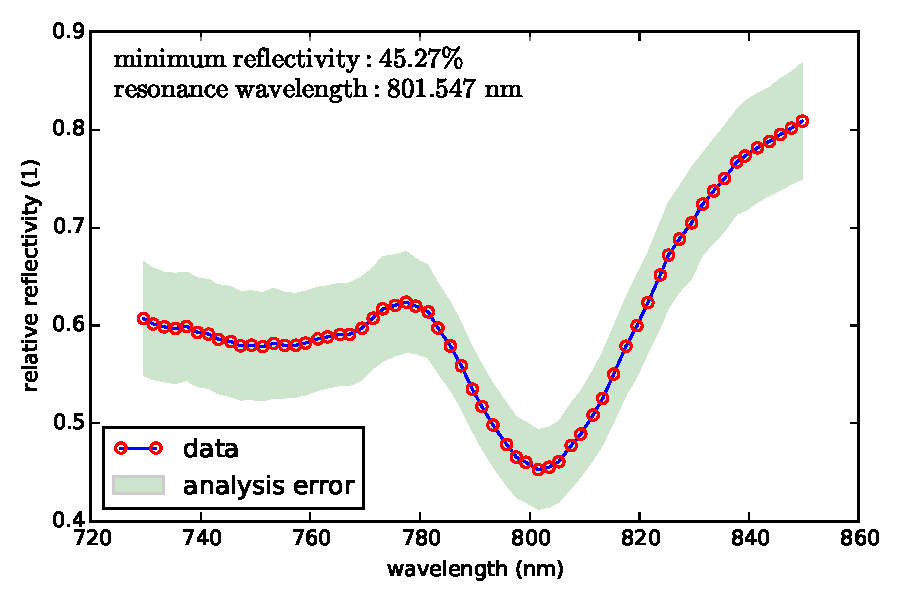
\includegraphics[width=0.47\textwidth]{reflectivity}
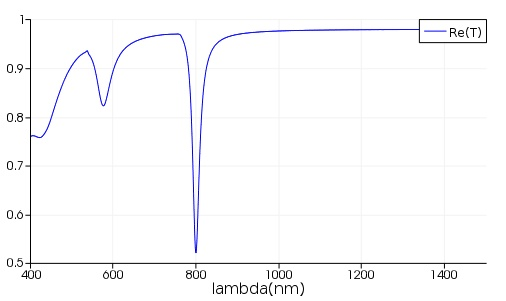
\includegraphics[width=0.43\textwidth]{Ag_sim}
\caption{\label{fig:Ag-b}
银纳米小孔阵列晶片的反射率谱。左图:反射率谱仪测得的反射率谱;右图:Lumerical FDTD 所模拟的实际加工参数下晶片的反射率谱。注意两图的横座标波长范围不同。}
\end{center}
\end{figure}

\section{NPC 参数的高功率实验测量}
完成离线反射率测量后,我们将 Ag NPC 晶片放入微波电子枪中进行了高功率实验,以检验其作为光阴极的表现。高功率实验中需评价的参数有:量子效率 QE(266\,nm 激光下),多光子光电发射电子产额/曲线(800\,nm 激光下)以及纳米表面的发射度。

为了将银晶片放入电子枪,采用了 cathode-plug 设计,即在铜阴极盘中心加工一个直径略小于晶片直径的孔,将银晶片从后端顶入阴极盘并压紧。微波电子枪中阴极盘和银晶片的相对位置见图 \ref{fig:Ag wafer}。
\begin{figure}[htbp]
\begin{center}
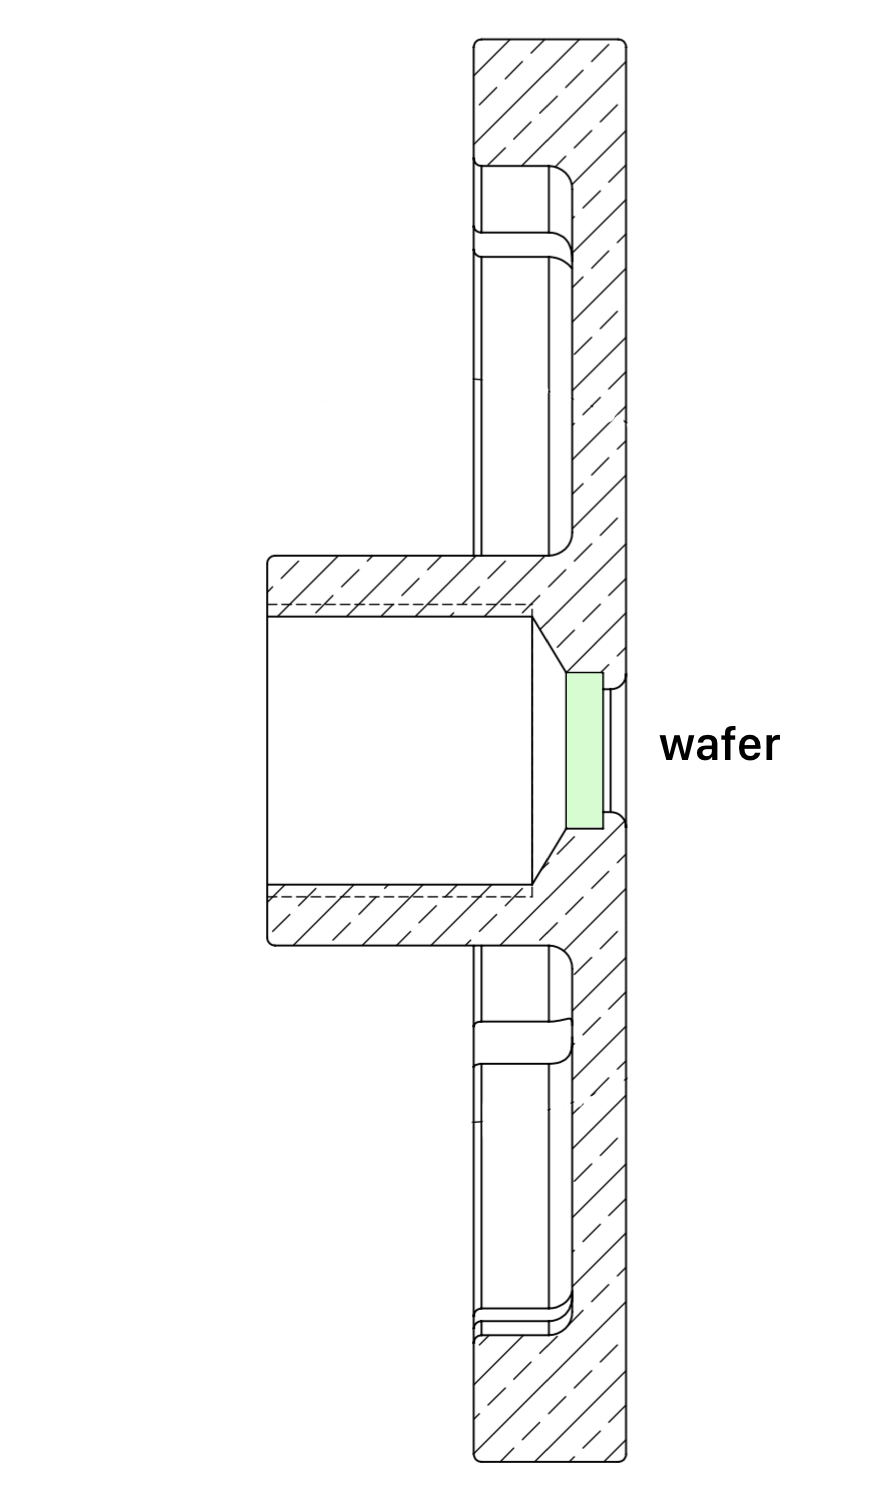
\includegraphics[width=0.23\textwidth]{cathodeplug.png}
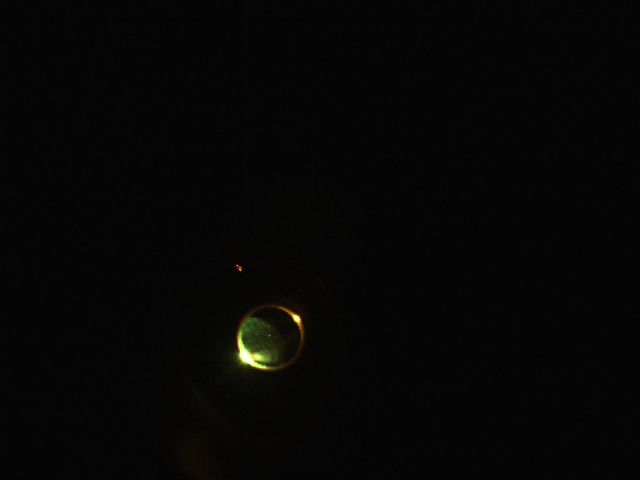
\includegraphics[width=0.5\textwidth]{wafer.png}
\caption{\label{fig:Ag wafer} 
左图:有 cathode-plug 设计的阴极盘截面示意图。绿色区域表示银晶片插入位置。右图:Ag NPC 晶片放入微波电子枪后从观察孔观察的形态。图像中的环清晰地显示了银晶片的边界,中央区域的绿色小点就是加工的纳米结构所在位置。}
\end{center}
\end{figure}

高功率实验在 UCLA Pegasus 实验室的束线上进行。束线的结构如图 \ref{fig:pegasus} 所示。
\begin{figure}[htbp]
\begin{center}
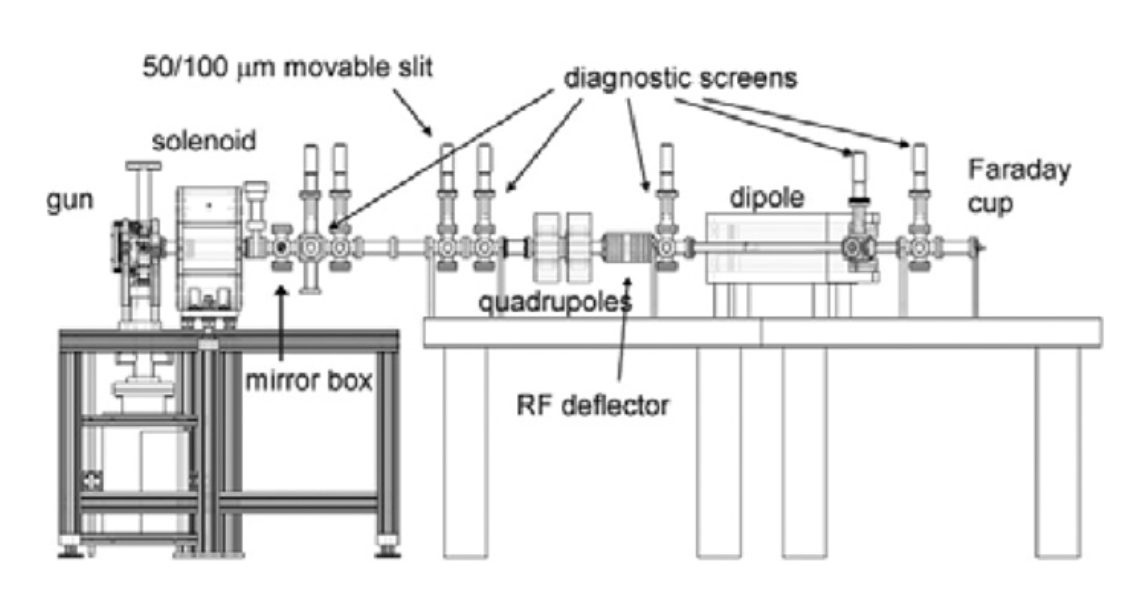
\includegraphics[width=0.9\textwidth]{pegasus.png}
\caption{\label{fig:pegasus} UCLA Pegasus 束线布局图。}
\end{center}
\end{figure}

\subsection{QE 测量}
首先在 266\,nm 的 UV 激光下测量了 Ag 晶片的量子效率 QE。为提高测量精度,采用了三种测量方法来校准电荷量:
\begin{itemize}
\item 利用束线末端的法拉第桶上的电压信号直接计算,公式为 $Q = \eta_FU_F$,其中 $\eta_F=1/15\,\text{pC/mV}$,$U_F$ 是法拉第桶上的电压信号,$Q$ 为束团电荷量
\item 对用来测量束团能量分布的能谱仪的图像进行积分作为相对电荷量,这种方法测量的电荷量需要用法拉第桶法的测量结果进行校准
\item 将束线尾部的 YAG 屏 2 号(用来测量电子束的横向尺寸与分布)上的图像进行积分,并用法拉第桶测量结果进行校准
\end{itemize}
我们采用了光电二极管来测量激光能量,设从光电二极管上采集到的电压信号为 $U_P$,那么激光能量 $E$ 可写做:$E = \eta_PU_P$,其中 $\eta_P=1/35\,\mu\text{J/mV}$。

实际测量中,需要改变激光脉冲能量,并记录每个脉冲能量对应的法拉第桶、能谱仪以及 YAG 屏 2 号的信号和图像。实验中 能谱仪和 YAG 屏的增益并不相同,分别为 1000 和 600,这个因素需要在对图像积分时进行考虑。实测的激光束团的能量损失率大约是 35\%(即从激光能量计测量位置传输到阴极的过程中激光的能量损失)。计算 QE 的公式如下:
\begin{equation}
\label{eq:QE}
\text{QE} = \frac{h\nu}{e}\cdot\frac{Q}{(1-R_{\text{loss}})E} = \frac{h\nu}{e}\frac{\eta_F}{(1-R_{\text{loss}})\eta_P}\cdot\frac{U_F}{U_P}
\end{equation}
其中 $h$ 是普朗克常数,$e$ 是电子电荷量,$R_{\text{loss}}$ 是激光能量损失率,其余参数意义与之前所定义的相同。图 \ref{fig:QE} 显示了 QE 的测量结果。从图中可看出 QE 大约是 $2.2\times 10^{-5}$,这和期望值比较接近。

\begin{figure}[htbp]
\begin{center}
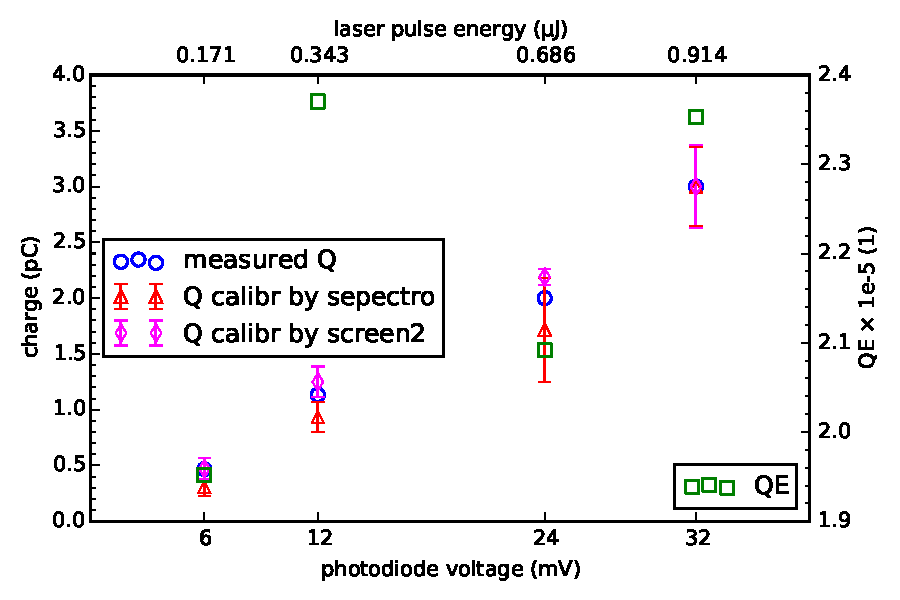
\includegraphics[width=0.6\textwidth]{photodiode}
\caption{\label{fig:QE} QE 测量结果。测量电荷量时采用了三种方法进行交叉比对。}
\end{center}
\end{figure}

\subsection{电子产额扫描}
由于只有多光子效应下,NPC 的优势才足够明显,电子产额测量在 800\,nm 激光下进行。测量方法如下:保持激光脉冲的能量为常量,使用激光扫描整个银晶片,对于每个扫描点,对 YAG 2 上的图像进行分析后提取出电子束束斑并积分,该积分值就是相对电荷量。实验中采取了两轮扫描,第一轮采用矩形格点进行全表面粗扫,之后在纳米结构附近采用矩形格点进行细致扫描。将激光位置与计算的相对电荷量进行对应,就可以获得电子产额扫描图。扫描结果见图 \ref{fig:qemap}。
\begin{figure}[htbp]
\begin{center}
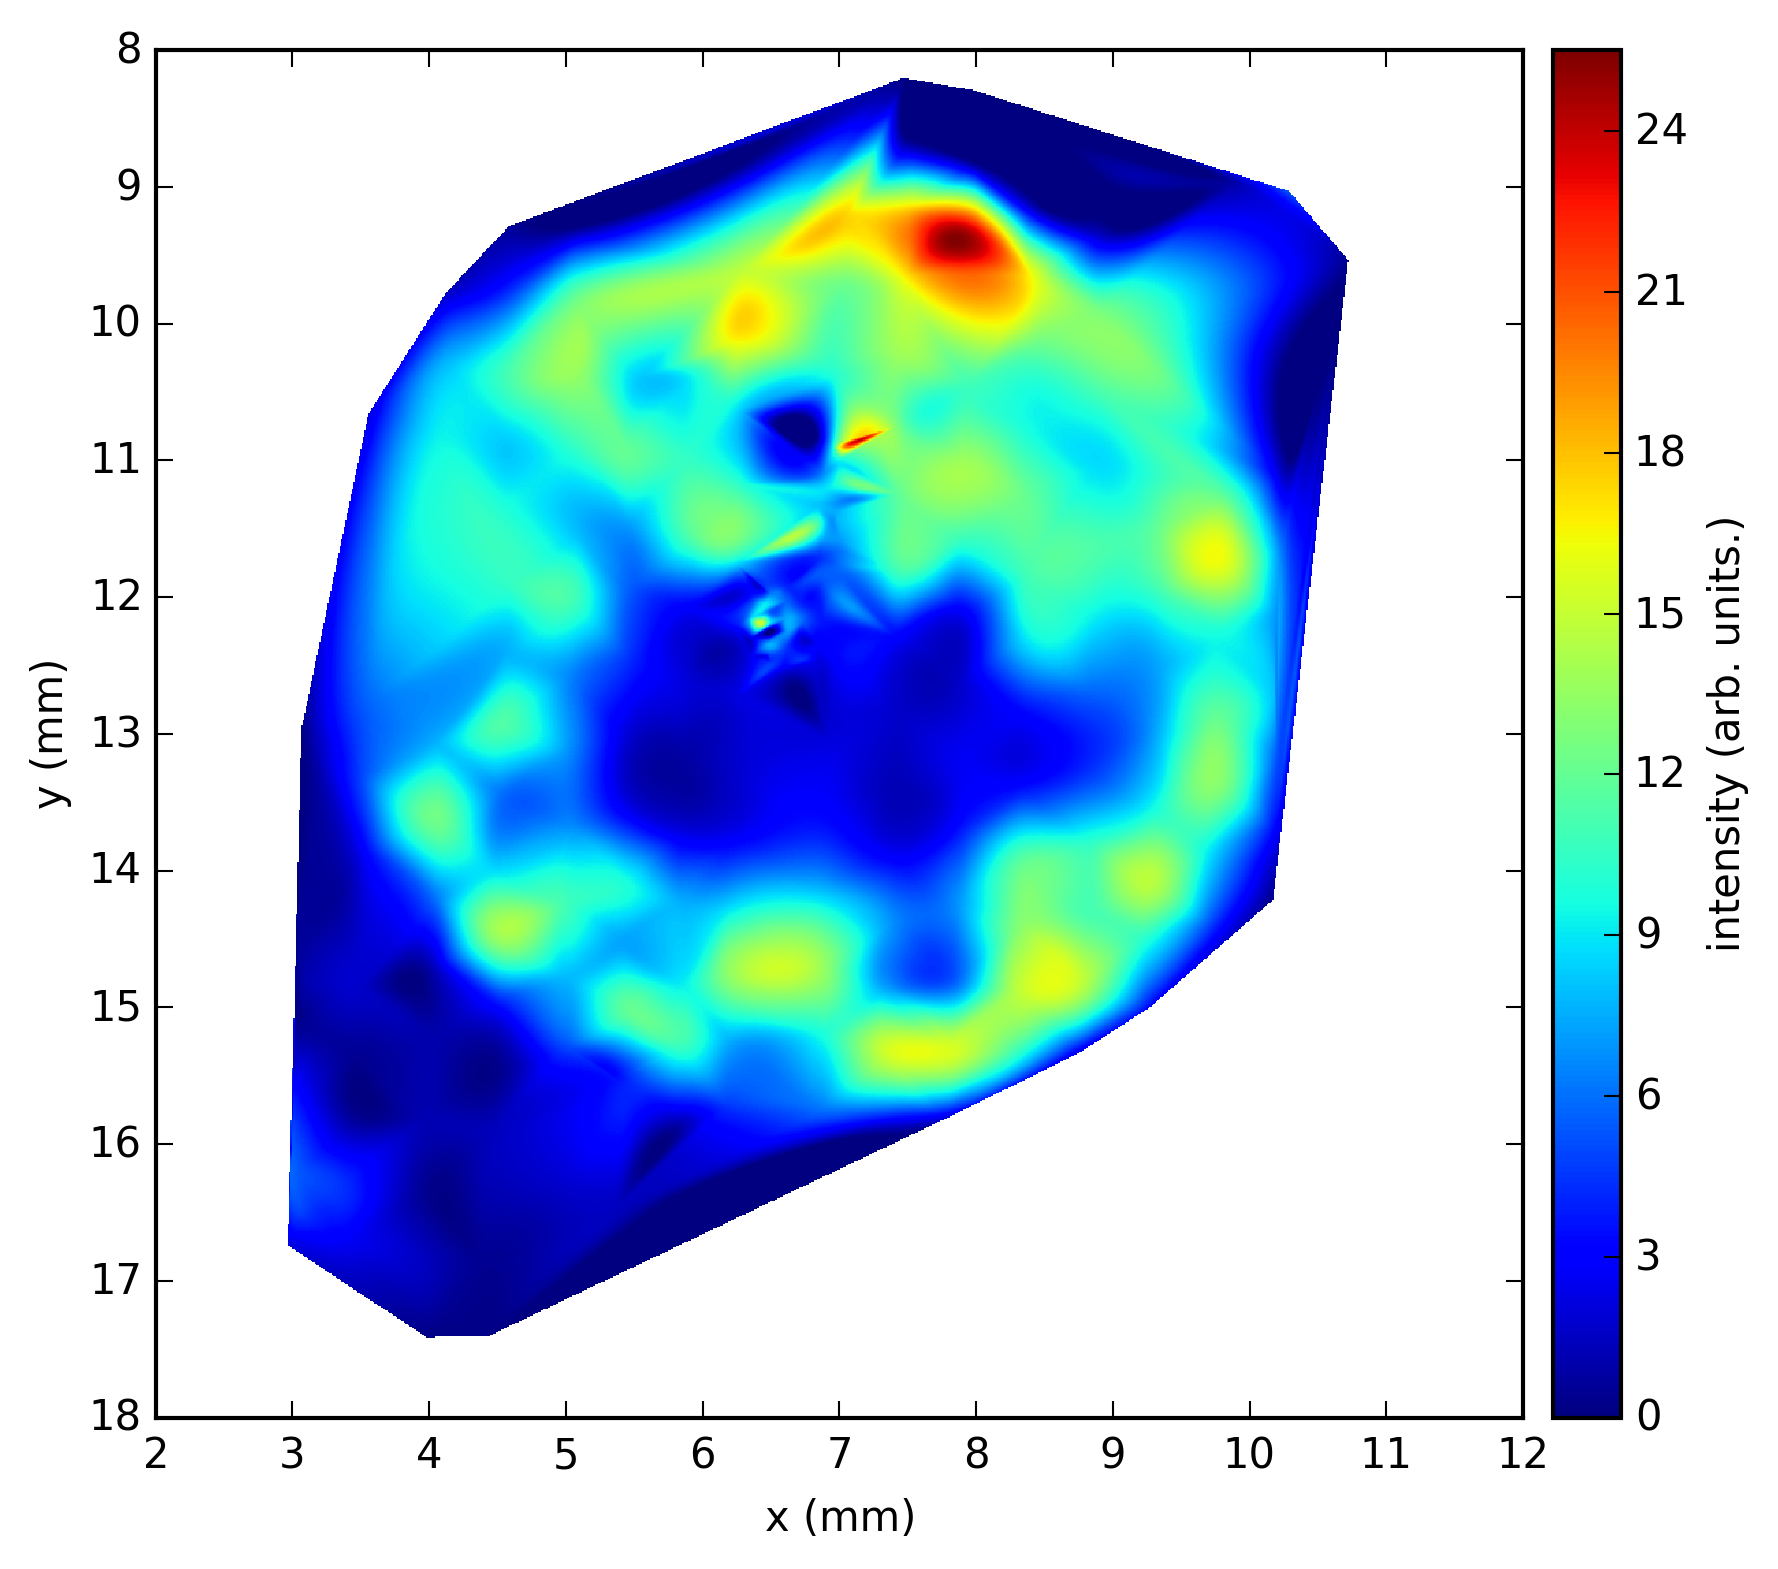
\includegraphics[height=0.6\textwidth]{qemap.png}
\caption{\label{fig:qemap} 电子产额扫描结果。该实验在 800\,nm 激光下进行,图中环状的高增益区域揭示了银晶片与铜阴极盘交界位置。}
\end{center}
\end{figure}

根据之前的离线反射率谱测量结果,银晶片表面的结构与 800\,nm 激光谐振,且对于银而言,800\,nm 激光主要会激发三光子光电效应,因此期待纳米结构所在的晶片中心区域有很高的电子产额。然而图 \ref{fig:qemap} 中可见,中心区域的电子产额增益只是 10 左右,远远小于 Pegasus 实验室较早的关于铜纳米阴极的结果(铜纳米阴极的电子产额增益近 3000)。考虑到实验中所用的激光尺寸要比纳米结构尺寸大,较低的产额增益可能是卷积的结果(即高增益部分和低增益部分的均值)。

SEM 测量给出银纳米结构的尺寸在 0.2\,mm 左右,而实验中所用激光横向尺寸在 1.3\,mm 附近,因此如果平均的电子产额增益为 10,那么银纳米结构的电子产额增益应为 $(10\times1.3^2-1\times(1.3^2-0.2^2))/0.2^2 \sim 400$,这个结果尽管依然较铜纳米阴极的结果低,但由于加工时相对于优化尺寸的误差,也是预期之中的。

图 \ref{fig:qemap} 中还可以观察到一个有趣的现象,即环状的高增益区域。该环的尺寸和银晶片的尺寸吻合,因此该现象说明银晶片与铜阴极盘交界处有很高的电子产额增益。此现象可以解释如下:

\subsection{多光子光电发射曲线}
将电荷密度 $\sigma$ 和吸收激光功率密度 $I$ 的关系画在对数坐标中,就得到所谓多光子光电发射($\sigma$-$I$)曲线\cite{Girardeau-Montaut:1993aa,Kupersztych:1994aa}。该曲线理论上是直线,其斜率就是多光子光电发射的阶数。银晶片的多光子光电发射曲线见图 \ref{fig:key}。
\begin{figure}[htbp]
\begin{center}
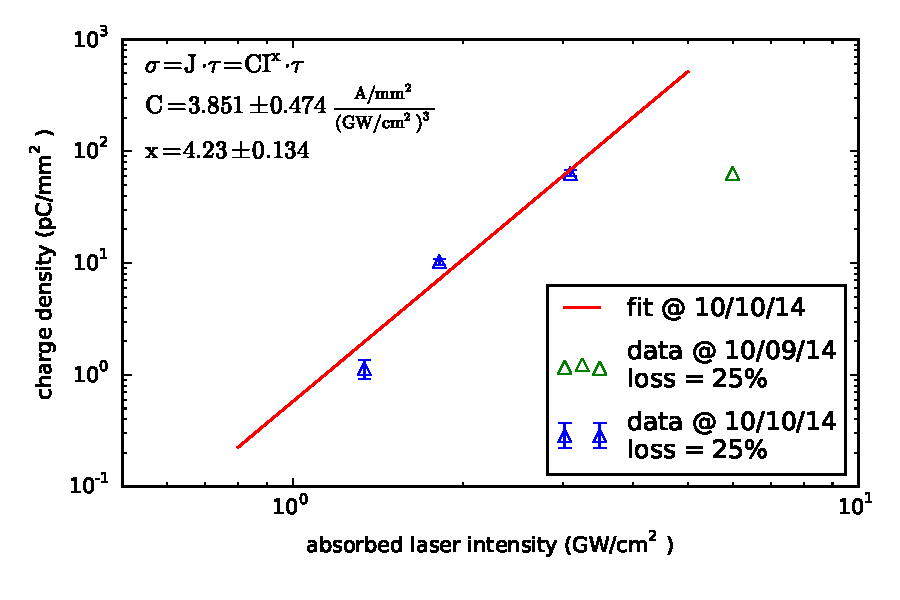
\includegraphics[width=0.6\textwidth]{keyplot}
\caption{\label{fig:key} 
多光子光电发射曲线。激光脉冲能量的传输损失因子为 25\%,实验中测量的银晶片的光滑部分发射率为 92\%。}
\end{center}
\end{figure}

实验中测量了三个数据点,通过拟合得到多光子光电发射曲线。拟合结果表明,在相同的吸收激光功率密度下,银阴极的电子产额要比铜阴极的高\cite{Li:2013aa}(银晶片的拟合曲线有更高的系数 $C$),这个结果符合单晶银逸出功($\sim$ 4.14\,eV)比多晶铜逸出功($\sim$ 4.31\,eV)更低的事实。

\subsection{发射度测量\label{ssec:emit}}
银晶片的发射度测量采用螺线管扫描法\cite{Ross:1987aa},测量时所用激光波长为 800\,nm。发射度测量实验布局见图 \ref{fig:layout},其测量结果见图 \ref{fig:emittance}。

值得注意的是,由于 cathode-plug 的设计,银晶片表面与铜阴极盘表面有一个小的距离(1.5\,mm),这会造成银晶片表面最大场强下降至正常情况的 2/3。该场强下降造成的问题讨论如下:

\begin{figure}[htbp]
\begin{center}
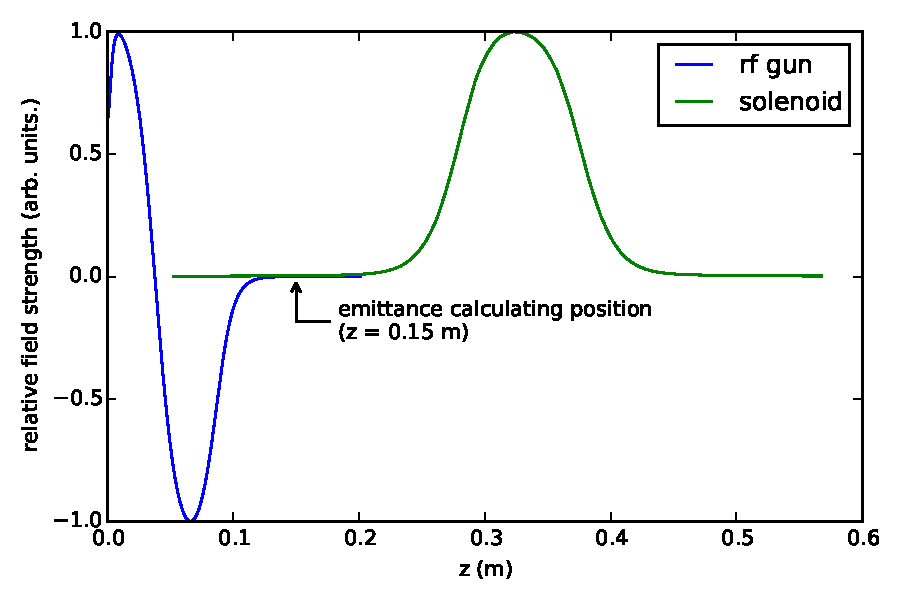
\includegraphics[width=0.6\textwidth]{layout}
\caption{\label{fig:layout} 
发射度测量布局图。蓝色曲线是归一化微波电子枪轴线电场,绿色曲线是归一化螺线管线圈强度。}
\end{center}
\end{figure}

从图 \ref{fig:emittance} 中展示的发射度测量结果以及实验中所用的激光横向尺寸可知,银纳米阴极的归一化热发射度分别是 1.6\,mm$\cdot$mrad/mm(x 方向)和 1.7\,mm$\cdot$mrad/mm(y 方向),这大概是平滑铜阴极归一化热发射度($\sim$ 0.8\,mm$\cdot$mrad/mm)的两倍,同时也比之前的铜纳米阴极归一化热发射度($\sim$ 1.4\,mm$\cdot$mrad/mm)\cite{Li:2013aa}略大。这个结果是符合直觉的,因为银纳米阴极正是牺牲了发射度以换取更大的电子产额增益。由于银纳米阴极的发射度相对较大,可能并不适合应用于对发射度有严格要求的应用(如 FEL),但是依然可以作为有潜力的电子源用于对电荷量要求高但对发射度要求不严格的应用,例如应用于尾场加速器中。
\begin{figure}[htbp]
\begin{center}
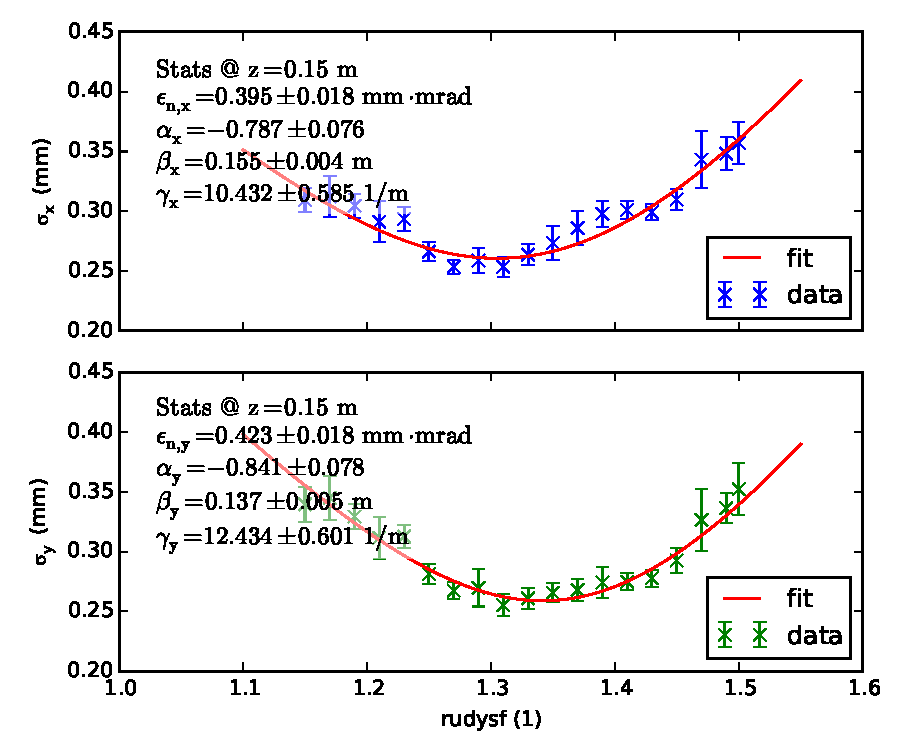
\includegraphics[width=0.6\textwidth]{emittance}
\caption{\label{fig:emittance} 
Ag NPC 的发射度测量结果。上图:x 方向发射度;下图:y 方向发射度。}
\end{center}
\end{figure}

\section{实验中一些现象的分析\label{sec:misc}}
\subsection{高功率下的纳米表面结构损伤}
\begin{figure}[htbp]
\begin{center}
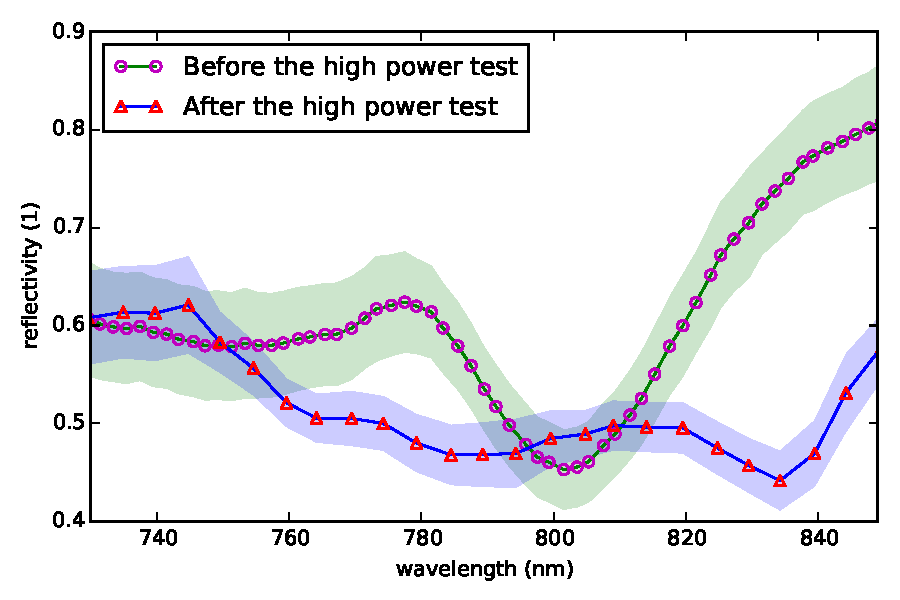
\includegraphics[width=0.6\textwidth]{silver_reflectivity_comparison}
\caption{\label{fig:afterhighpower} 高功率实验前后的银纳米结构的反射率谱对比。}
\end{center}
\end{figure}

高功率测试结束后,我们将银晶片从电子枪中取出并再次进行了离线反射率谱测量。高功率实验前后的反射率谱对比见图 \ref{fig:afterhighpower}。

图 \ref{fig:afterhighpower} 中明显可见,800\,nm 处的谐振峰消失了,且近乎全波段的发射率都有所下降。这个现象说明在高功率测试中,银纳米阴极的结构被破坏了(结构被破坏导致无法再与 800\,nm 光共振,且更加粗糙的表面使得反射更接近漫反射,从而整个波段的反射率都有所下降)。

由于在多光子光电发射曲线测量中所使用的激光功率密度最高,我们有理由猜测该结构的破坏就是发生在多光子光电发射曲线测量实验中。这也同时说明尽管银纳米阴极的电荷产额较铜更高,却也有比铜更低的损伤阈值。银纳米阴极具体损伤阈值有待进一步实验测量。

\subsection{cathode-plug 设计导致的问题}
正如节 \ref{ssec:emit} 中提到的,银晶片表面场由于 cathode-plug 导致的晶片与阴极盘不共面而有大幅下降。为了研究不共面可能带来的问题,我们对晶片与阴极盘表面不同间距下的阴极表面场下降因子(有间距时表面场强与无间距时表面场强之比)进行了数值模拟。模拟结果见图 \ref{fig:comp}。
\begin{figure}[htbp]
\begin{center}
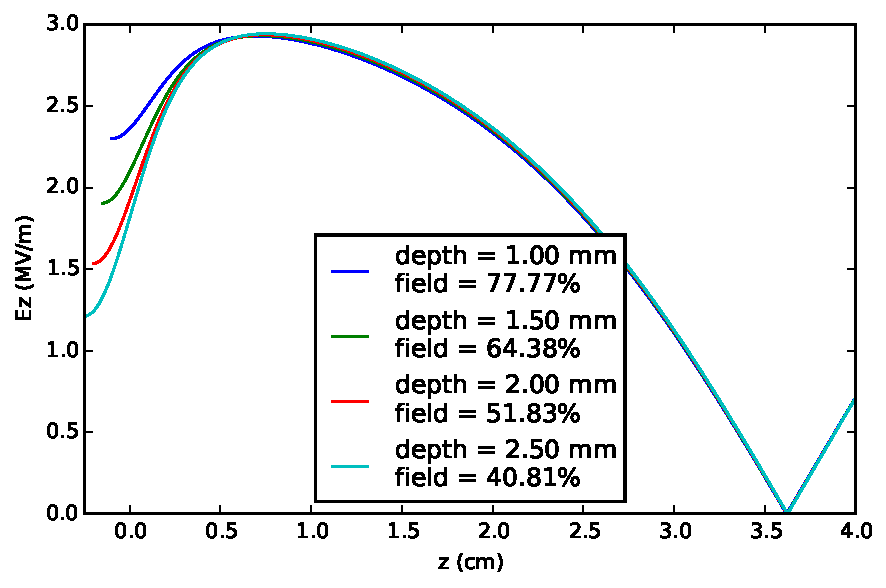
\includegraphics[width=0.6\textwidth]{comp2}
\caption{\label{fig:comp}
晶片与阴极盘表面不同间距下半腔中的轴线场强分布。z 轴零点代表铜阴极盘表面所在位置。}
\end{center}
\end{figure}

在 cathode-plug 设计中,晶片与阴极盘间距(晶片深度)是 1.5\,mm,因此场下降因子在 64\% 左右。阴极表面场强的降低会导致电子枪发射相位的偏移(进而造成枪出口处的能散增加),同时对于大电荷量的发射情形,也会由于对空间电荷力的抑制降低而使发射度增长。晶片与阴极盘间距的存在也会显著提高晶片边缘的电场强度,从而导致了银晶片与铜阴极盘交界处的高电子产额增益。

晶片深度造成的另一个问题是电子枪工作频率的偏移。晶片深度为 1.5\,mm 时,电子枪中 $\pi$ 模的工作频率从 2855.60\,MHz 漂移到 2855.99\,MHz($\Delta f=386.7\,\text{kHz}$)。工作频率漂移可以通过调整铜阴极盘形状来补偿。
\begin{figure}[htbp]
\begin{center}
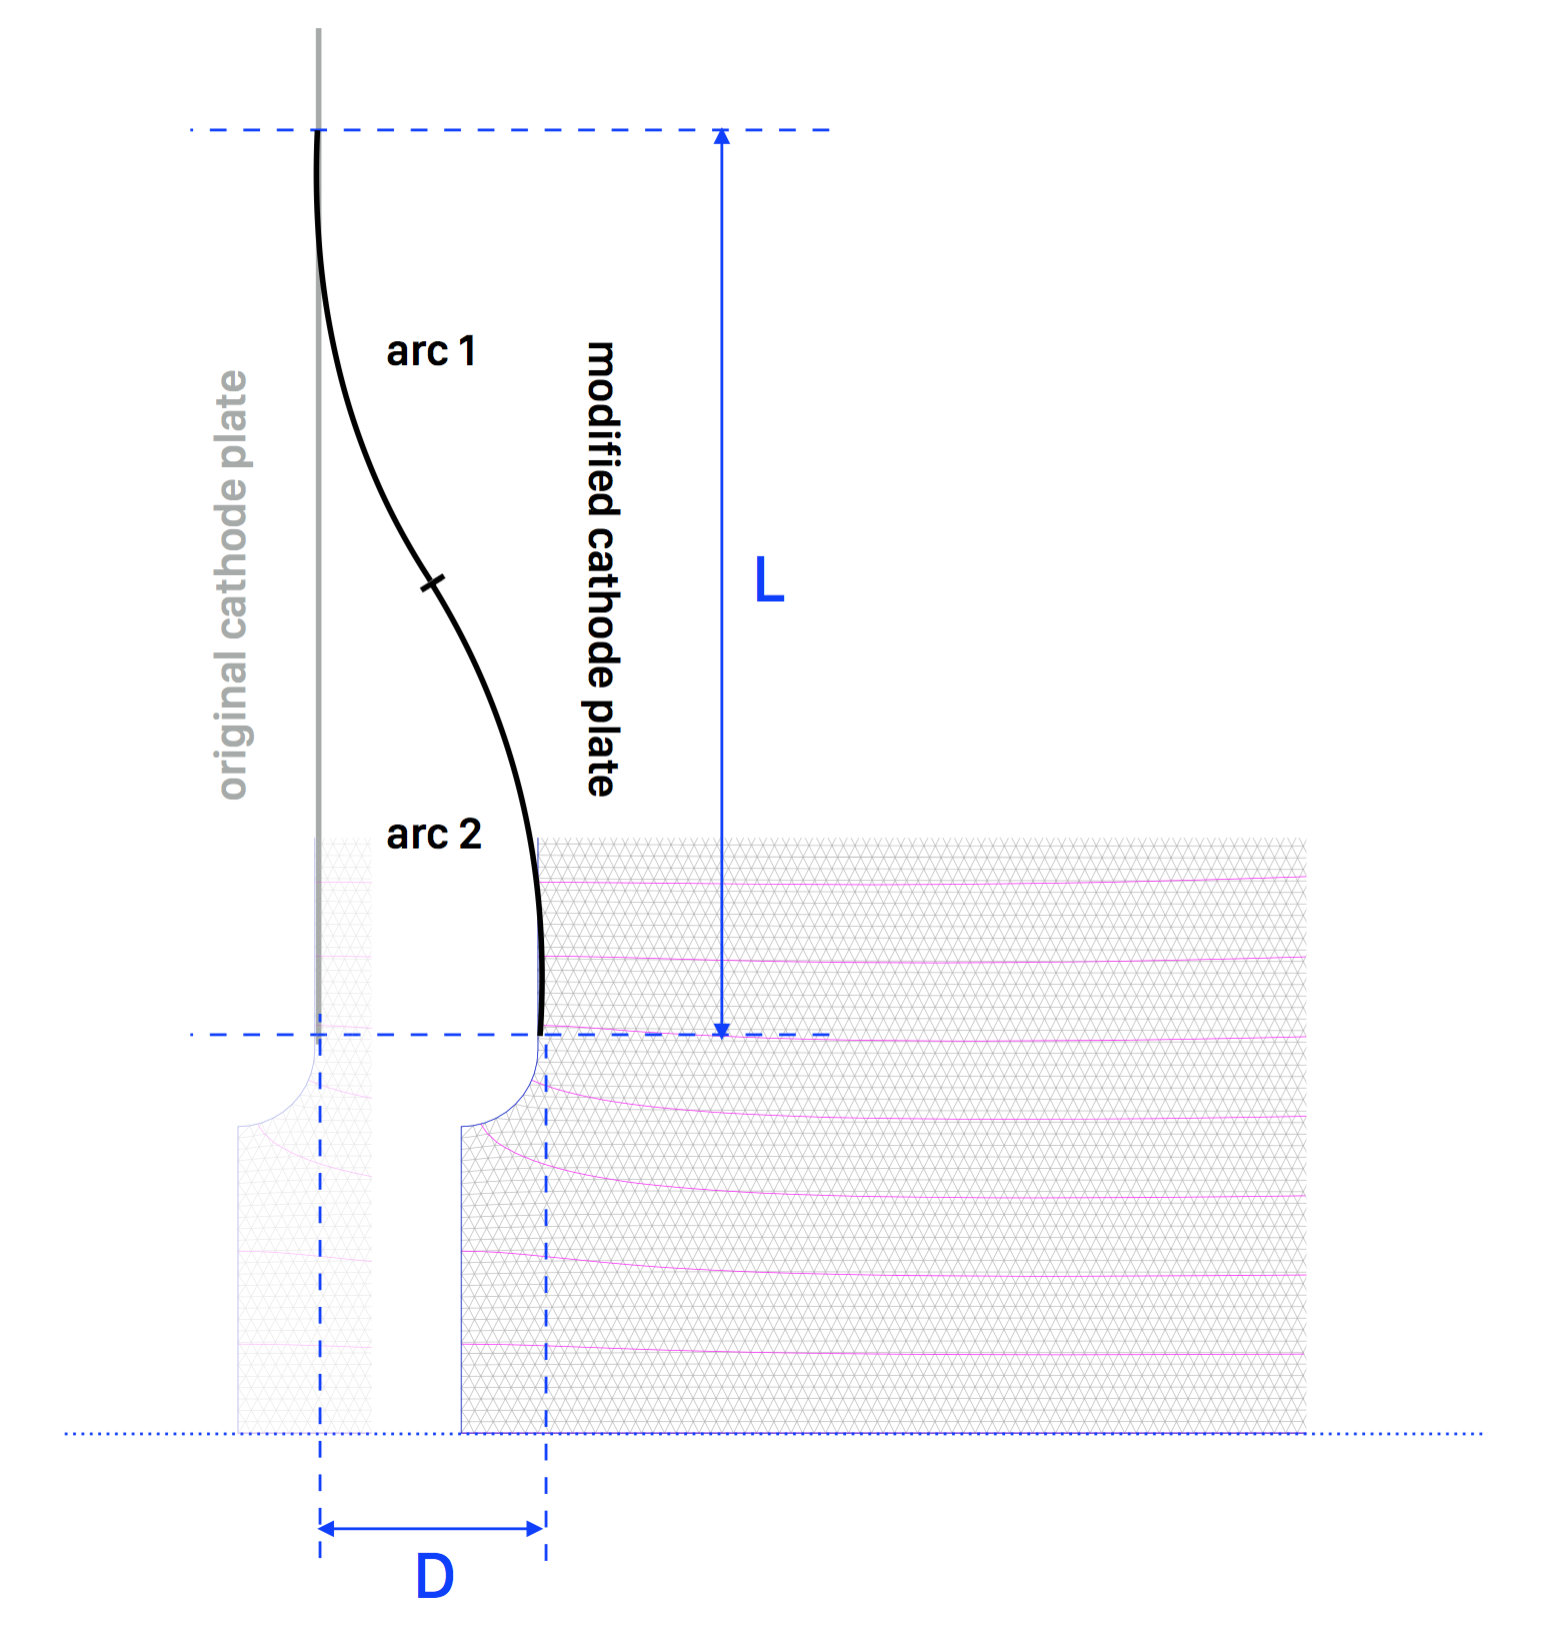
\includegraphics[width=0.6\textwidth]{modify}
\caption{\label{fig:mod} 为补偿频率漂移的调整过后的铜阴极盘轮廓示意图。}
\end{center}
\end{figure}
如图 \ref{fig:mod} 所示,我们引入了两条全同的圆弧段,两条圆弧反对称相连形,在阴极盘上形成一个缓变坡度。当 $L=10\,\text{mm}$,$D=0.12\,\text{mm}$ 时,电子枪的工作频率就被补偿回到 2855.60\,MHz。

\subsection{离线宽带反射谱仪测量结果中 600\,nm 处谐振峰的分析}
在对银晶片等 NPC 阴极进行离线反射率谱的测量过程中,我们在 600\,nm 附近观察到了一个谐振峰,然而 Lumerical 的模拟中却并未给出这个峰。对此现象我们有下面解释:

简单地说,反射率谱上 600\,nm 附近的峰是由宽带反射率谱仪的工作原理造成的。在离线反射率谱测量中,被测量的并不是绝对反射率,而是相对反射率:我们采用 $\text{Brightness}_{\text{pattern}}/\text{Brightness}_{\text{background}}$ 作为纳米结构的反射率,但是背景(银晶片的光滑部分)的反射率并不是 1 而是永远小于 1,因此绝对反射率会比测量值要小。同时由于反射率谱仪是宽带的而非单频的,纳米结构或者背景的亮度是入射光各频率分量贡献亮度的平均值。基于上面分析,相对反射率可以被写为下面形式:
\begin{equation}
\label{eq:refl}
\bar{R}_{\text{relative}}(\lambda) = \dfrac{\bar{R}_{\text{pattern}}(\lambda)}{\bar{R}_{\text{flat}}(\lambda)} = \dfrac{R_{\text{pattern}}\ast f_{\text{spectrum}}(\lambda)}{R_{\text{flat}}\ast f_{\text{spectrum}}(\lambda)}
\end{equation}
其中 $f_{\text{spectrum}}$ 是入射光的能谱。600\,nm 处谐振峰的产生原因在图 \ref{fig:reason} 中进行了说明,详细的解释请参见图 \ref{fig:reason} 标题中的说明文字。
\begin{figure}[htbp]
\begin{center}
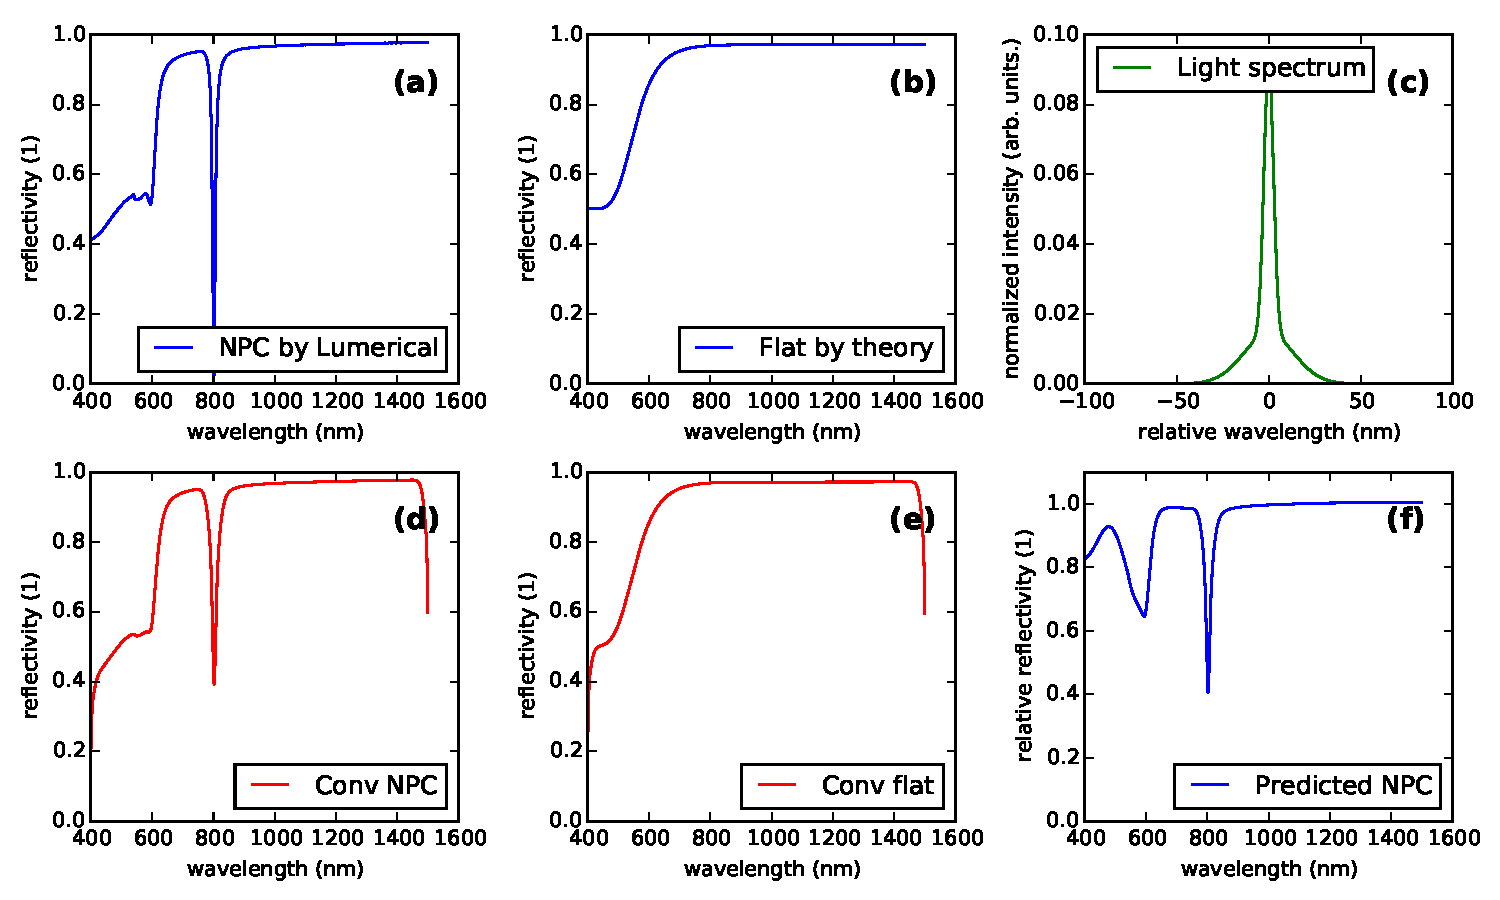
\includegraphics[width=0.9\textwidth]{comparison}
\caption{\label{fig:reason} 600\,nm 处谐振峰的成因。(a):Lumerical 给出的模拟曲线,注意此时 600\,nm 处并没有谐振峰;(b):应用 Fresnel 定律计算了阴极平滑表面的反射率,计算中需要的阴极材料的复折射率可在 \href{http://refractiveindex.info}{refractiveindex.info} 中找到。(c):假定入射光能谱可以写成两个高斯分布之和,根据实验测量,入射光能谱的 FWHM 是 6\,nm;(d):利用式 \ref{eq:refl},计算纳米阴极反射率与入射光能谱的卷积;(e):平滑金属阴极表面反射率与入射光能谱的卷积;(f):将(d)和(e)中两卷积曲线相除后得到的相对反射率曲线。可以看到,(f)中 600\,nm 处出现了明显的谐振峰。}
\end{center}
\end{figure}
预测曲线和实验测量曲线的差异可能是以下原因造成的:
\begin{itemize}
\item 实验中入射光能谱可能与假设不同
\item 实际纳米结构和在 Lumerical 中所模拟的结构(由于实际加工原因)可能不同
\item 实验中入射光可能非垂直入射
\end{itemize}

\section{小结\label{sec:sum}}
本章中,我们实验探究了表面纳米阴极作为高亮度光阴极候选的可能性。首先采用 Lumerical 数值模拟优化了不同材料(铜,镍,镁,银)的纳米结构尺寸;随后采用银晶片作为测试目标,应用宽带反射率谱仪对表面刻有纳米结构的银晶片进行了离线反射率谱测量,以验证实际纳米结构能够与 800\,nm 激光谐振;最后我们采用 cathode-plug 设计将银晶片放入电子枪中进行了高功率测试。在高功率实验中,测量了 266\,nm 激光下银晶片的量子效率 QE,在 800\,nm 激光下进行了银晶片的电子产额扫描,使用螺线管扫描法测量了 800\,nm 激光下的银晶片热发射度以及测量了银纳米结构的多光子光电发射曲线。

266\,nm 激光下银晶片的量子效率 QE 测量值是 2.2$\times10^{-5}$,800\,nm 激光下的电子产额增益约为 400,x 向和 y 向的归一化热发射度分别为 1.6\,mm$\cdot$mrad/mm 和 1.7\,mm$\cdot$mrad/mm。多光子光电发射测量表明相同激光功率密度下,银纳米阴极相较于铜纳米阴极可以产生更高的电荷密度,但同时热发射度也要比铜纳米阴极大约 15\%。与平滑铜阴极相比,热发射度高了近一倍。银纳米阴极的这一性质会对其在 FEL 等对发射度有严格要求的应用产生限制,但是其在需要大电荷量的应用(例如尾场加速)中依然是一个有潜力的选择。我们也讨论了实验中观察到的一些有趣现象,如高功率测试后银纳米结构的损坏,离线反射率谱测量中 600\,nm 处奇怪的谐振峰,电子枪中由于 cathode-plug 设计造成的一系列效应等等。
